\documentclass{llncs}
\usepackage[title]{appendix}
\usepackage[pagebackref]{hyperref}
\usepackage{subcaption}
\usepackage{graphicx}
\usepackage{comment}
\usepackage{amsmath,amssymb}
\usepackage{color}
\usepackage{float}
\newcommand{\reffig}[1]{\hyperref[#1]{Figure~\ref*{#1}}}
\newcommand{\refsec}[1]{\hyperref[#1]{Section~\ref*{#1}}}
\newcommand{\reftab}[1]{\hyperref[#1]{Table~\ref*{#1}}}
\newcommand{\refapp}[1]{\hyperref[#1]{Appendix~\ref*{#1}}}
\newcommand{\thickhline}{%
    \noalign {\ifnum 0=`}\fi \hrule height 1pt
    \futurelet \reserved@a \@xhline
}
\DeclareMathOperator*{\argminA}{arg\,min}

\begin{document}

\pagestyle{headings}
\mainmatter\def\ECCVSubNumber{100}
\title{Towards Bringing Together Numerical Methods for Partial Differential Equation and Image Processing}
\author{Stanislav Arnaudov, Markus Hoffmann}
\titlerunning{Towards Bringing Together Numerical Methods for Partial Differential Equation and Deep Neural Networks}
\authorrunning{Stanislav Arnaudov, Markus Hoffmann}
\institute{Karlsruhe Institute of Technology,\\Kaiserstrasse 12,76131 Karlsruhe, Germany\\ \url{http://www.kit.edu/english/}}

\maketitle

\begin{abstract}
  A central problem in the field of Computational Fluid Dynamics (CFD) is to efficiently perform a simulation of fluid flow while keeping the processing time low. Classical methods that provide accurate results, work based on partial differential equation solvers. They, however, require a considerable amount of processing time which is a problem when there are different simulation-parameter sets. We propose an alternative method for performing a simulation of fluid flow around an object based on convolutional neural networks (CNNs). We investigate a novel approach that uses simulation images as input for the CNN.\@ Several models are built, each trying to generalize a different subset of the parameters of the simulation. All models are based on the U-Net architecture and generate an image for the next time-step of the simulation. On average, the models perform an order of magnitude faster than the classical solvers at the cost of reduced accuracy. The generated images, however, are close enough to the real ones, so that a human observer can perceive them as the same. We also evaluate the results with appropriate error metrics.
\keywords{Computational Fluid Dynamics, Convolutional Neural Networks, U-Net, Image processing}
\end{abstract}

\section{Introduction}\label{introduction}
Computational Fluid Dynamics (CFD) is a field that deals with performing simulations of fluid flows. The task usually consists of setting certain initial conditions in a defined space and solving a large mathematical problem for each timestep of a given simulation. Two central points of interest in CFD are the processing time needed for a simulation and the accuracy of the results. It is clear that low processing time and high accuracy are desired but often a certain trade-off has to be made. With our research, we want to propose an innovative method for quickly inspecting the results of a simulation while keeping the accuracy high enough for them to make sense.

We've concentrated our study on 2D simulations of incompressible fluid flow around an object in a channel according to the Navier-Stokes equations~\cite{bistafa2018}. This setup has three adjustable parameters --- the inflow speed, the viscosity and the density of the fluid. The solutions of the simulation are three separate fields over the input space --- two velocity fields in $x$ and $y$ directions and a pressure field. These can be conveniently visualized as images over the input space. We are mainly interested in those image representations of the timesteps of the simulation. We call the image representations of the timesteps ``frames'' of the simulation. The sequence of these frames shows how the flow develops throughout the simulation.

Classical methods for performing such simulations are based on partial differential equations (PDEs) solvers. The simulation setup is first formalized as a mathematical model in the form of a time-dependent differential equation. In itself, this equation is then transformed and brought into a suitable for solving form. In a general case, basic technique that can be used is the finite difference method (FDM)~\cite{bashar2011,petersson2018,zhang2014,nahit2011}. This method can provide accurate results at the cost of large computational time. The generated results are in the form of raw numbers representing the velocities and pressure fields which have to be visualized separately. Our method aims to generate straight the visualizations while needing much lower computational time.

In recent years there has been a large interest in neural networks and their capabilities~\cite{krizhevsky2012,simonyan2014,zeiler2011,liu2017,ronneberger2015}. Convolutional Neural Networks (CNNs)~\cite{long2014} in particular have been successfully applied in a wide variety of contexts~\cite{eremeev2019,schulz2019,zhangyang2019,yang2019} and have proven to be a valuable tool. One of the major fields where the performance of CNNs is recognized is image processing. A lot of research has shown how CNNs can achieve state-of-the-art performance in tasks like image classification~\cite{xie2019,xie2016aggregated,he2015}, image segmentation~\cite{xie2016aggregated,choi2020cars} of image-to-image mapping~\cite{liu2017,radford2015,park2019}. With our research, we try to tie CFD and CNNs together and show how image processing approaches can be applied to performing numerical simulations.

In our work, we want to investigate how CNN can be used to generate an image of the simulation in interest. We build models that take an image from the previous timestep as an input and transform it into an image for the next timestep. The built CNNs can also take certain parameters of the simulation and transform the image in accordance with these parameters. With this approach, we are trying to transform the numerical task of calculating a timestep of simulation into an image processing task.

We base our work on the approach of~\cite{pix2pix}. In recent years GANs show impressive results in image generation~\cite{DashGALA17,ZhangXLZHWM16,karras2017progressive}. Conditional GANs (cGANs) extend these capabilities of the generator network and allow it to learn image-to-image translation tasks. We want to show how conditional GANs can be used in the context of numerical simulations. In this case, the generation of a frame of a simulation is conditioned on the previous frame of the same simulation.

The goal of our research is to see to what extent the described approach is viable. We achieve that by investigating how a cGANs generalizes the different parameters of the investigated simulation. Two subsets of the parameters are defined --- fluid parameters (kinematic viscosity and density) and the inflow speed of the fluid. For each of these two subsets, we train separate models and evaluate their performance in different use cases. A baseline model that does not take parameters into account is also built. We give more details on the models in \refsec{methodology}.

The built models are evaluated from two points of view. Firstly, as the output of the network is meant for a human observer, we evaluate the generated images based on their perceived fidelity. Secondly, as the networks try to model a numerical task, we also compare the real and generated images objectively by measuring the actual differences between them.

Because of the nature of our task, two evaluation cases are given. On the one side, we want to see how the networks perform while predicting individual images. That is, a network performs a single simulation timestep and the results of that are evaluated. On the other side, we also want to see how the inaccuracies in the predicted images can accumulate over time. Hence, we also evaluate the models by recursive application where the output of the network is used again as an input for a certain amount of timesteps. More details about the evaluations are given in \refsec{eval}.

Lastly, we briefly want to motivate why we propose exactly this approach. Images represent a well-defined input space as every pixel can take a limited range of values --- $[0, 255]$. This makes the handling of data in image form convenient. Based on the previous works, we assume that fully convolutional neural network can process information in this form more easily. Furthermore, convolutional neural networks are well-established models for performing image processing tasks. We were interested in how a numerical task can be turned into an image processing task as in certain situations, the image results have the priority.
We believe that this image processing approach can be used to generate a simulation image much faster than a numerical approach with some loss in accuracy. The accuracy loss is the subject of our research.

\section{Related Work}\label{related_work}
There has been a long-standing interest whether or not neural networks can be used in strictly mathematical contexts~\cite{neville2002,lample2019}. When it comes to differential equations,~\cite{lagaris1998} has demonstrated for the first time how neural networks can be applied to solve PDEs and ODEs by designing a loss function based on a particular equation. More recently, a similar approach has been presented in~\cite{avrutskiy2017}. With the emergence of deep learning~\cite{krizhevsky2012}, DNNs have been successfully applied in numerical tasks as well~\cite{wei2017,battaglia2016}. By flow problems, CNNs have been successfully applied in analyzing and calculating properties of flow fields~\cite{georgiou2018} and enhancing the quality of low-resolution simulations~\cite{tempoGan} while fully connected networks have helped in liquid splash modeling~\cite{hu2017}. 

In CFD, DNNs have been used in a wide variety of contexts. Turbulence models have been developed in~\cite{beck2018},~\cite{pfeiffer2019} has developed a network that predicts the motion of organs during operation and~\cite{tompson2016} uses a highly tailored neural network to solve Euler equations for fluid flow and thus accelerate the simulation process~\cite{thuerey2018} solves the problem of the Reynolds-Averaged Navier-Stokes (RANS) simulation similarly to us. They do not use cGANs, do not target the image representation of the simulation and tackle different equation from us but they too try to map initial conditions to a solution through an end-to-end model. Our approach is not exactly comparable to the one of~\cite{thuerey2018} as we are considering a different numeric problem (the Navier-Stokes equations). Also,~\cite{thuerey2018} tries to map the boundary conditions of the problem to the solutions. We, on the other hand, map a solution of the studied simulation to the next one.

The Navier-Stokes equations have also been a point of interest with respect to neural networks.~\cite{raissi2018} models the motion of particles in a fluid through a specifically designed network that encodes physical principles based on the Navier-Stokes equations.~\cite{baymani2010} has derived a trial solution of the equations in terms of a neural network. In contrast to these works, we aim at using a model with general architecture and applied it to a specific numerical simulation while approaching the problem from image processing point of view.~\cite{guo2016} deals with a similar problem by trying to predict the stabilized state of a laminar flow using a general model. The task, however, does not require the recursive application of the model but a single one.

By now, the image-to-image translation through CNNs is well established and has found numerous applications~\cite{zhao2020,liu2017,ZhangXLZHWM16,park2019}.~\cite{pix2pix} has specifically stated how the ``community-driven research'' has popularized their work by applying it in different ways~\cite{Moschoglou2019,Kim2020,Chen2019}. We see our work as a demonstration of how cGANs can also be applied to numerical simulation context.

\section{Methodology}\label{methodology}
The task is to build a network that can predict the next frame of the simulation based on the previous one. Each frame represents a timestep of the simulation and consists of a three-channel image. Two of the channels encode the velocity fields in both directions and the third channel is the pressure field of the fluid. We are interested in how the usage of the pressure field affects the performance of the built models. Therefore, for each model two variants are trained --- one that uses the pressure field and one that does not.

We did not construct a single holistic model that can handle all of the simulation's parameters. Our efforts are concentrated on building a couple of smaller ones that take into account subsets of the parameters. The studied models are:
\begin{list}{$\circ$}{}
\item[$\cdot$] a constant model --- does not take into any of the parameters and it is trained with data from a single simulation. It is conceived as a baseline and proof of concept model that is there to show how a neural network can learn to generate simulation timesteps in from of images.
\item[$\cdot$] A fluid inflow speed model --- the model receives the inflow speed of the fluid as an extra input. It is trained with data from several simulations with different inflow speeds.
\item[$\cdot$] A viscosity and density model --- the model receives the viscosity and density of the fluid as extra inputs.
\end{list}
By evaluating each model we want to see how a network can generalize each of the parameter subsets and to what extent.

\subsection{Simulation Setup and Data generation}
\emph{To study the performance of the models on predicting frames of a concrete simulation, we generated the training data ourselves. In what follows we give details about the process.} The training data was generated by performing numerous simulations of incompressible fluid flow around a rectangular object in a channel. The simulations were modeled according to the Navier-Stokes equations for incompressible flow. Because we are interested in the image representations of the simulations, we are dealing only with the 2D case. Several boundary conditions describe the simulation setup:
\begin{list}{$\circ$}{}
\item[$\cdot$] Inflow condition on the left side of the channel
\item[$\cdot$] Outflow condition on the right side of the channel
\item[$\cdot$] No-slip condition on the bottom and top side of the channel as well as the sides of the object.
\end{list}
The simulation setup has three separate adjustable parameters --- inflow speed $g$, fluid density $\rho$ and fluid kinematic viscosity $\nu$.

We generated three sets of simulations for training the three kinds of models.
\begin{list}{$\circ$}{}
\item[$\cdot$] constant: a single simulation with $\rho=0.2, \nu=0.0009, g=1.5$.
\item[$\cdot$] varying inflow speed: $40$ simulations with different inflow speed. The inflow speeds are in the range of $[1.5,4.0]$ with a step of $0.0625$.
\item[$\cdot$] varying viscosity and density of the fluid: $324$ simulations all with different fluid viscosity and density. The viscosity was in the range of $[0.003, 0.0009]$ with a step of $0.0000064$ and the density was in the range of $[1.0, 10.0]$ with a step of $0.028$. We used the product of the two-parameter ranges to perform simulations with all of the possible combinations between the two parameters.
\end{list}

The choice of concrete values for the parameters is deliberate. All of the values are chosen so that the Reynolds number~\cite{trinh2010critical} of the simulations in the range of $[90, 450]$. This causes a transitional flow with vortex shedding effect. We were interested whether the built models can predict the emerging \emph{Kármán vortex street}~\cite{karaman1911} behind the object in the channel. Thus the Reynolds numbers were chosen so that the effect can occur.

The simulations were performed numerically by solving the differential equation describing the flow --- the Navier-Stokes equation. This was done with a numerical solver library --- \emph{HiFlow}~\cite{gawlok2017} ---  that works on the base of the Finite element method~\cite{strang2008analysis}. The solver supports parallelization with \emph{MPI}~\cite{mpi} and \emph{OpenMP}~\cite{dagum1998openmp} and we used 12 MPI processes to run each simulation. For all of the simulations, the timestep for of solver was set to $0.035$ seconds. This means a single time step of the simulations corresponds to a $0.035$ seconds of physical time.

The numerical solver on itself cannot be used to render the simulation results to images. For this reason, we used \emph{ParaView}~\cite{ahrens2005} to load the simulation data and exported it as a sequence of images in \emph{PNG} format. We opted out for using grayscale images as early experiments with RGB-images did not deliver satisfying results. We used the default ``Grayscale'' color preset of ParaView to visualize the results. Each frame of the simulation was exported as three separate grayscale images. Finally, the images were cropped to select a subset of the space that contains the object and space behind it.

Because the number of simulations in each set is different, we also generated a different number of images per simulation based on the corresponding set. For the constant dataset, we rendered $1904$ frames of the simulation ($66$ seconds of simulated physical time). For the inflow speed dataset --- overall $10050$ frames coming from the $40$ simulations ($335$ frames per simulation for $12$ seconds of simulated physical time). For the viscosity-density model --- overall $104328$ frames from $334$ simulations ($322$ frames per simulation for $11$ seconds of simulated physical time). Even though the simulations in the different datasets represent different time intervals, they are all long enough to develop the flow patterns that we are interested in.

After all of the images were generated, a test-train split was created for each of the datasets. The split for the inflow speed and viscosity-density sets were done manually. For the inflow speed set, we selected every fourth simulation to be part of the test set and for the viscosity-density set --- every 25th. All other simulations are used for training. The split for the constant dataset was done at random. All of the splits result in  80\% of the data being used for training and the rest for testing. It is important to note that all of the images in the test sets come from simulations with parameters that are not found for the simulations in the training sets. This means that the datasets are designed in a way to see if the models can generalize the parameters of the simulations and predict simulations with parameters that are unseen during the training.

\subsection{Training approach and networks details}
We base our generative models almost entirely on~\cite{pix2pix}. We use the conditional GAN approach to train a generator network that can perform image-to-image translation. As explained in~\cite{pix2pix}, the traditional GAN method uses a random vector $z$ as in input to the generator network $G$ to generate output $y$, $G:z \rightarrow y$. Conditional GANs also feed an input image $x$ to the generator, $G: x,z \rightarrow y$.~\cite{pix2pix} and~\cite{wang2016} suggest that in certain cases the usage of $z$ can be usefully but we decided not to include for our generator as we want a deterministic network. The discriminator network is modeled with the function $D:x,y \rightarrow v$ that evaluates the likelihood of $y$ being a real image. To note is that the discriminator network has access to the real image $x$ and tries to guess, if $y$ is the real or generated output.

We adopt the objective for the discriminator network and we modify it slightly by leaving out the random vector $z$.
\begin{equation}
  \mathcal{L}_{cGAN} (G, D) = (\mathbb{E}[\log D (x,y)] + \mathbb{E}[\log D (x, G(x))])/2 \\
  = (\log D (x,y) + \log D (x, G(x)))/2
\end{equation}
where $x$ is the input image and $y$ is the target image. We leave out the expected value calculation as we do not use the random vector $z$ in our objective. In contrast to unconditional GANs, both the generator and the discriminator network have access to the input image. The objective is divided by two to slow down the training of the discriminator relative to the generator as suggested by~\cite{pix2pix}.

The objective for the generator network is comprised of two parts --- the value of the discriminator as well as a $L1$ distance loss between the target and the predicted images. According to~\cite{pix2pix} the $L1$ loss promotes less blurring and captures the low frequency details of the images. The $L1$ loss is given by:
\begin{equation}
\mathcal{L}_{L1} (G) = \mathbb{E}[\left\lVert y - G(x)\right\rVert_1]
\end{equation}
The final object for the generator is thus:
\begin{equation}
G^* = \argminA_G \max_D \mathcal{L}_{cGAN}  + \lambda \mathcal{L}_{L1} (G)
\end{equation}
For all of the models we used $\lambda = 100$ as done in~\cite{pix2pix}. We also experimented with lower values for $\lambda$ but results were not as good.

\noindent\textbf{Networks Architectures:} For our generator we use the U-Net~\cite{ronneberger2015} variant proposed in~\cite{pix2pix}. It is a standard encoder-decoder~\cite{hinton2006} model with skip connections between parts of the encoder and the decoder. We also experimented with ResNet~\cite{he2015} based generator but the results were not satisfactory. Our networks use blocks of layers of the from convolution-normalization-ReLu~\cite{batchnorm}. The encoder-decoder first downsamples the input till a bottleneck layer is reached and what follows is an upsampling to the original size of the input image.

For the discriminator, we follow the method of~\cite{pix2pix} and we use their PatchGAN discriminator network.\@ This is a convolutional network that classifies patches of the input as real or predicted. To not is that the whole image is given as an input. The majority of the results in~\cite{pix2pix} show that a patches of size $70\times 70$ yield the best results but in our case, the experiments showed otherwise. We, therefore, we opted out for using patches of size $286\times 286$ pixels.

\noindent\textbf{Training details:} We train the described three models with the generated datasets. When loading the images in memory, we first resize them to an appropriated for a network size of $1024\times 256$ (width $\times$ height). We then apply random crops as well as add random noise to each channel of the images. We do this to force the generator to learn the actual features of the simulation and make over-fitting harder. Before the images are fed into the networks, we also multiply them with a mask of the object in the channel. This is an image that has zero value in the area where the object is located and values of one for every other location. The multiplication with the mask results in an input image with values of zero in the area of the object. The predicted images are also multiplied with the mask. This procedure lets us examine how well the network generates the pixels in the places that we are interested in --- the places where the flow occurs. The object mask itself is also given as an input to the generator network. This gives the network the information of where the object is. This information cannot be embedded in the other input images as the zeroed values in the location of the object are interpreted as velocity values by network.

Two of the models also take certain simulation parameters as inputs. In all cases, the parameters are real values. In order for the network to be able to use them as part of the input, we transform these values in constant single-channel images with a value equal to the corresponding parameters. This means that for each simulation parameter there is an extra channel in the for the generator network. Thus, depending on the model being trained, the network can take anywhere between 3 --- velocity fields and object mask --- and 6 --- velocity and pressure fields, object mask and two parameter channels --- channel input. The output of the generator, however, can either be 2 or 3 channel image depending on whether the pressure field is used or not.

For the training procedure, we follow the standard approach proposed in~\cite{goodfellow2014}. With each mini-batch, we first optimize the discriminator and then the generator with the discussed objectives. We use Stochastic Gradient Descent~\cite{kiefer1952} with the Adam optimizer~\cite{kingma2014} with a learning rate of $0.0002$ and standard momentum parameters $\beta_1=0.9$ and $\beta_2=0.999$. The used batch size for the constant and inflow speed models was set to $3$ and for the viscosity-density models to $4$. Those are relatively small numbers for batch sizes but~\cite{pix2pix} suggests that the U-Net architecture benefits from small batches in image-to-image translation problems. Our experiments confirmed this.

Because of the differences in the amount  of data available for training each model type, suitable epoch numbers were chosen for each of them. The constant models were trained for $45$ epochs, the inflow speed models for $30$ epochs and the viscosity-density models for $10$ epochs.

All of the models were trained and evaluated on a single Nvidia GTX 980Ti GPU.\@ The implementation of the models was done in the \emph{PyTorch}~\cite{paszke2017automatic} python library for machine learning.

\section{Evaluation}\label{eval}
\noindent\textbf{Evaluation Metrics:} When it comes to the evaluation, we have two separate views on the results generated by the models.

On one hand, we are dealing with image data that is meant to be perceived by a human observer. This implies that full accuracy is not essential and therefore we place the importance on the perceived qualities of the predicted frames. This makes sense as in our case a human is concerned with the general development of the simulation over time. Under those considerations we have chosen appropriate metrics to compare the predicted simulation images with the real ones. In this aspect, the first of the metrics is \emph{Peak Signal to Noise Ratio} (PSNR). It is related to the Mean Squared Error (MSE) and it is given by
\begin{equation}
PSNR = 10 \cdot \log_{10}\left(\frac{255^2}{MSE}\right)
\end{equation}
PSNR is measured in decibel (dB) and it is a common metric used to evaluate lossy compression algorithms~\cite{psnr1,psnr2}. It measures the difference between the original and reconstructed images and considers the visual fidelity of the reconstruction. This makes the metric suitable in our case. Typical PSNR values of lossy image and video compression algorithms are between $30$ and $50$ dB. Higher PSNR values are desired, as the value of PSNR is inversely proportional to the value of MSE.

When considering the perceived image quality, we also have decided to use correlation to compare the predicted and the real simulation frames. We think that if the predicted images differ only in a factor from the real ones, the models can accurately capture the relative difference between the pixels of the target image. For this reason, we opted for also evaluating the results through statistical correlation between the predicted and the real images. Naturally, we want to see if the models can generated images with correlation close to $1.0$.

On the other hand, as we are dealing with a numerical task, we also wanted to evaluate the results more objectively. Classical solvers are evaluated in terms of the actual differences between the real and generated result and not the perceived differences. For those reasons, we have chosen two more metrics --- average absolute difference and maximal absolute differences. We calculate them based on differences between the corresponding pixels of the predicted and the real simulation frames. Both metrics are then averaged across the test set and are given in percentual values. The evaluation with these metrics should represent how well our models perform the simulation in the context of a CFD system. As their are both difference measures, lower values are desired for these metrics.

\noindent\textbf{Evaluation Details:}
\emph{In this subsection, we want to give several details on the training and evaluating approach.}
\begin{itemize}
\item[$\cdot$] All models were trained from scratch and no pretraining or transfer-learning was undertaken.
\item[$\cdot$] For each model, the whole training and evaluating procedure was done ten times with different seeds for the random number generators of our python scripts. We report the results of each run and give them in a form of error plots or explicitly give the standard deviation of all runs.
\item[$\cdot$] All of the reported results for the individual runs are averaged across the simulation frames in the training sets.
\item[$\cdot$] While performing the experiments, we did not tweak the hyperparameters of the models excessively. We did, however, tried several sets of hyperparameters until the models achieved satisfactory results. The exact hyperparameters are given in \refapp{app1}.
\end{itemize}

\noindent\textbf{Single Image Performance:}
As mentioned before, we have two evaluation strategies for the models. The first of them is to see how well a single frame of the simulation is predicted. In this case, we feed all of the simulation frames in the test set to the network and evaluate the predicted frames.

\reffig{fig:single_psnr} shows the results of the different model types with respect to PSNR.\@ Examples of the predicted images are given in \reffig{fig:single_images}. We can clearly see that the predicted images are almost identical to the real ones. In all cases, we measured a correlation of about $0.9998$ so we will not give it explicitly here. We think that the images themselves illustrate the high correlation.

\reftab{tab:single} summarizes the results of the evaluation with the average and maximal difference metrics.

The effects of the usage of the pressure field can be seen in the variance of the results. The pressure field has the potential to make the models better but in some runs, it can also make them worse. We believe this is the case because the pressure fields increase the complexity of the data but it also carries information about the simulation that can be useful for the networks.

Based on our experiments, we can say that achieving good performance was the hardest for the constant model. We attribute that to the limited data with which it was trained --- only a single simulation. Contrary to the intuition, the more varied data is easier to predict, as it can be seen in the results for the inflow speed and viscosity-density models. We also believe that a bigger test set can better estimate the performance of our models. This probably also contributes to the worse results for the constant models.

\begin{figure}
  \begin{subfigure}{.3\textwidth}
    \centering
    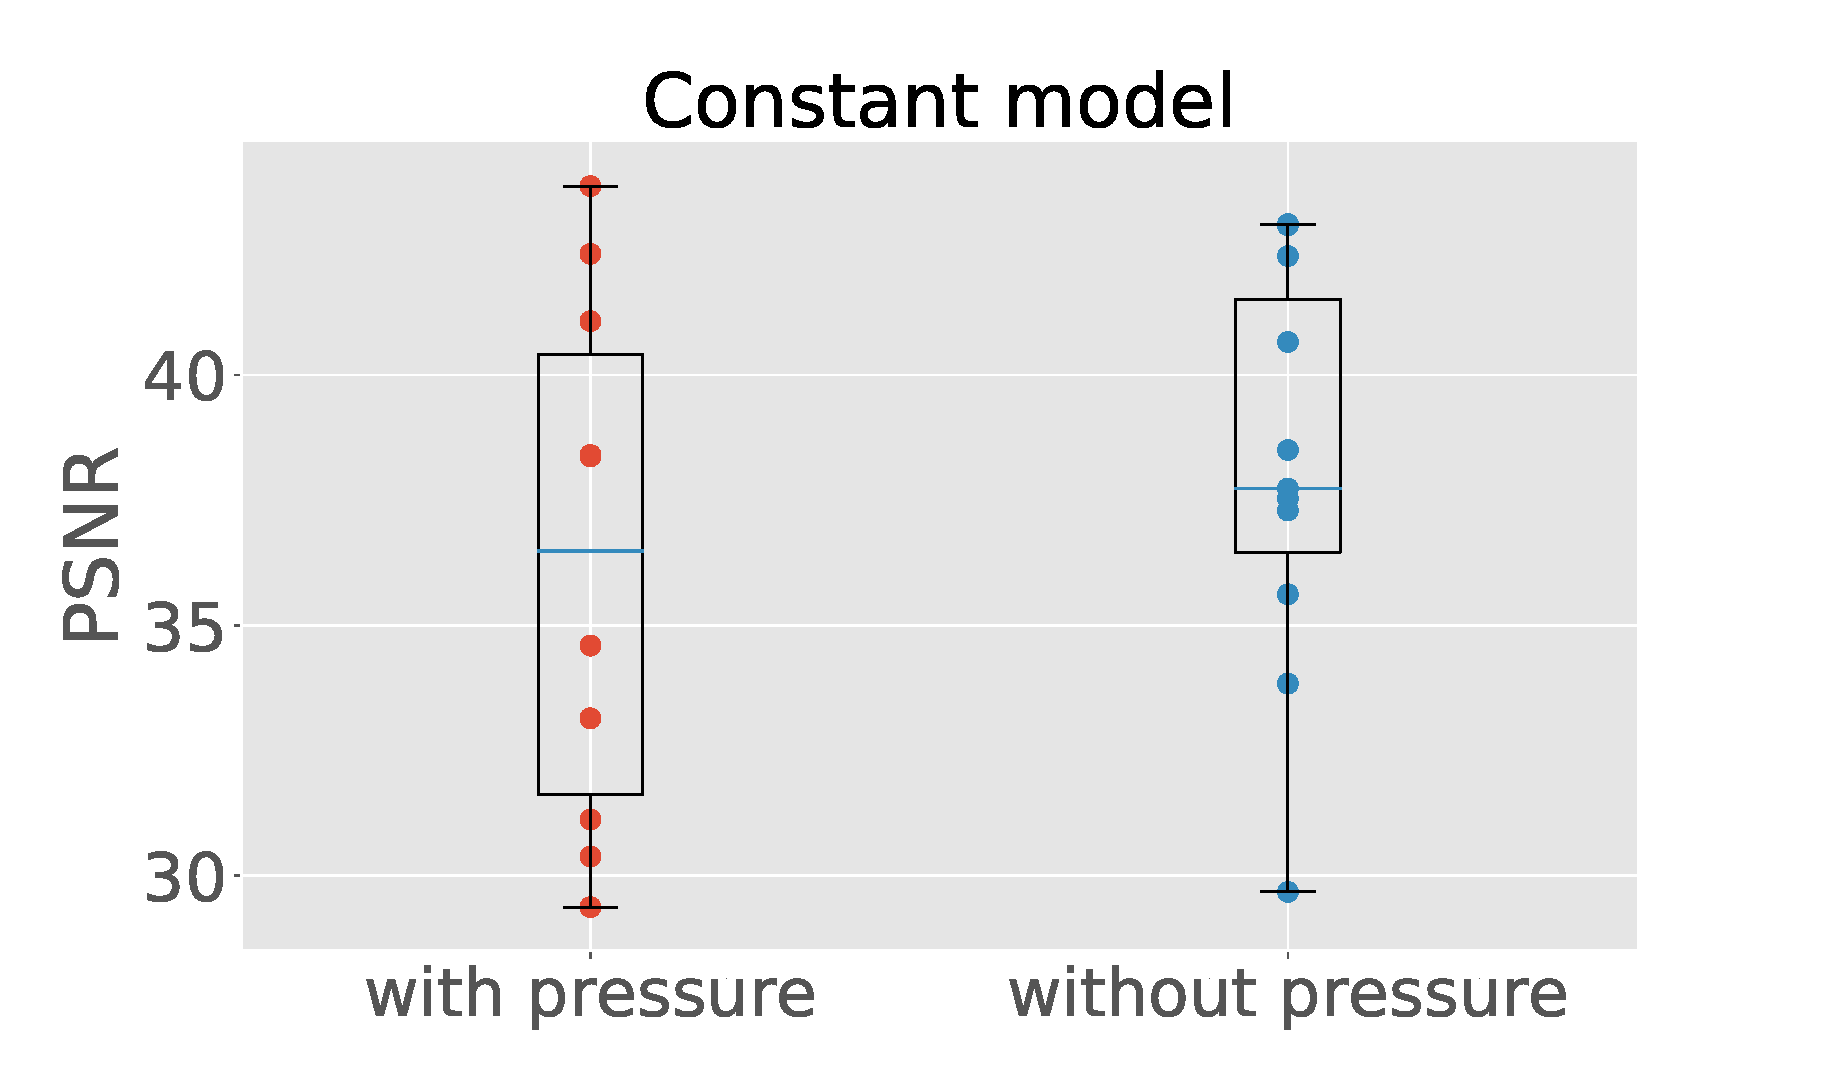
\includegraphics[width=1\linewidth]{imgs/charts/single_const_psnr}
  \end{subfigure}
  \begin{subfigure}{.3\textwidth}
    \centering
    \includegraphics[width=1\linewidth]{imgs/charts/single_speed_psnr}
  \end{subfigure}
  \begin{subfigure}{.3\textwidth}
    \centering
    \includegraphics[width=1\linewidth]{imgs/charts/single_fluid_psnr}
  \end{subfigure}
  \caption{The evaluation samples for the constant model show how inconsistent its performance can be. We assume this is due to the limited data that the consent model uses. In contrast to that, we see how the viscosity-density model achieves significantly higher average PSNR.\@ On the other hand, the usage of the pressure field decreases the performance of the viscosity-density model. The may be because of the overall complexity of the model. The pressure field only adds another component to it that makes it even more hard to train.}\label{fig:single_psnr}
\end{figure}

\begin{table}
  \begin{center}
    \begin{tabular}{lcc|cc}
      \textbf{Model type} & \multicolumn{2}{c|}{\textbf{Max difference(\%) }}  &  \multicolumn{2}{c}{\textbf{Average difference(\%)}}\\
      \hline 
      \multicolumn{3}{c|}{}&&\\
                 & \underline{With pr.} & \underline{without pr.}  &  \underline{With pr}.& \underline{without pr.}\\
      
      Constant           &14.56(1.97)&44.04(18.73)&0.60(0.29)&0.72(0.54)  \\
      Inflow speed       &32.16(0.55)&45.68(1.21)&0.55(0.05)&0.93(0.07)   \\
      Viscosity-density  &57.00(42.46)&14.70(2.65)&13.85(13.43)&0.37(0.09)\\
    \end{tabular}
  \end{center}
  \caption{All of the given numbers are in percents. In the parenthesis we also give the standard deviation of the corresponding metric.}\label{tab:single}
\end{table}

\begin{figure}
  
  \begin{subfigure}{.5\textwidth}
    \centering
    \large{x-velocity}
    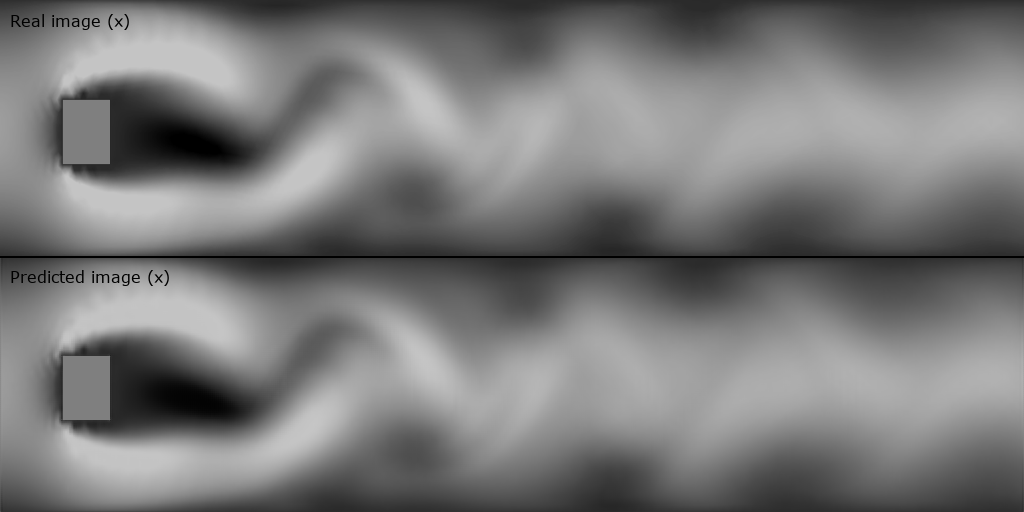
\includegraphics[width=1\linewidth]{imgs/single_constant_x}
  \end{subfigure}
  \begin{subfigure}{.5\textwidth}
    \centering
    \large{y-velocity}
    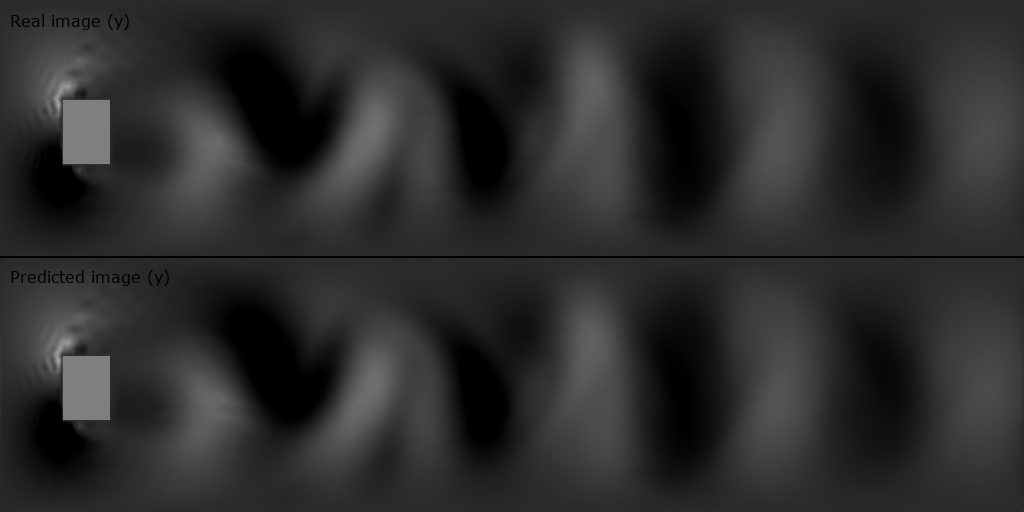
\includegraphics[width=1\linewidth]{imgs/single_constant_y}
  \end{subfigure}
  \begin{center}
    Constant model
  \end{center}

  \begin{subfigure}{.5\textwidth}
    \centering
    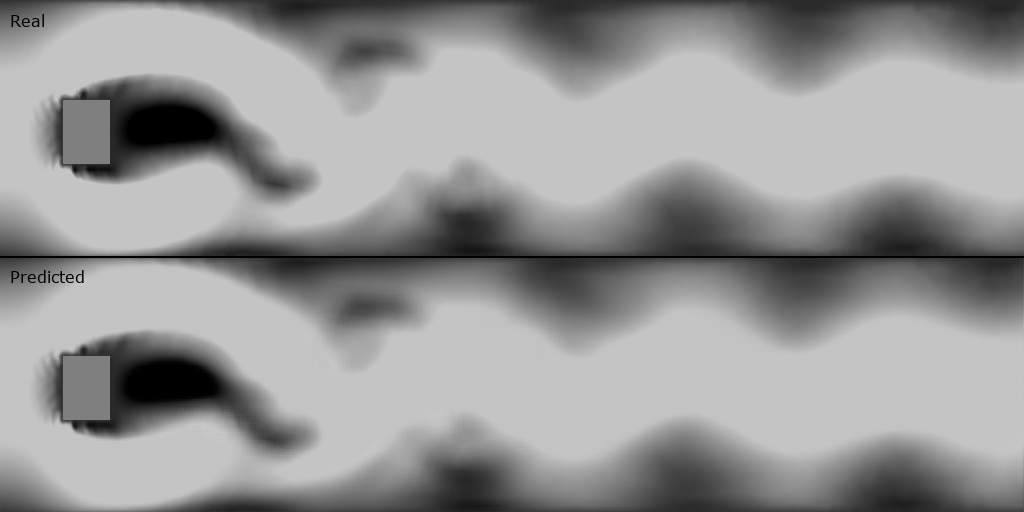
\includegraphics[width=1\linewidth]{imgs/x_recursive_0_speed_8}
  \end{subfigure}
  \begin{subfigure}{.5\textwidth}
    \centering
    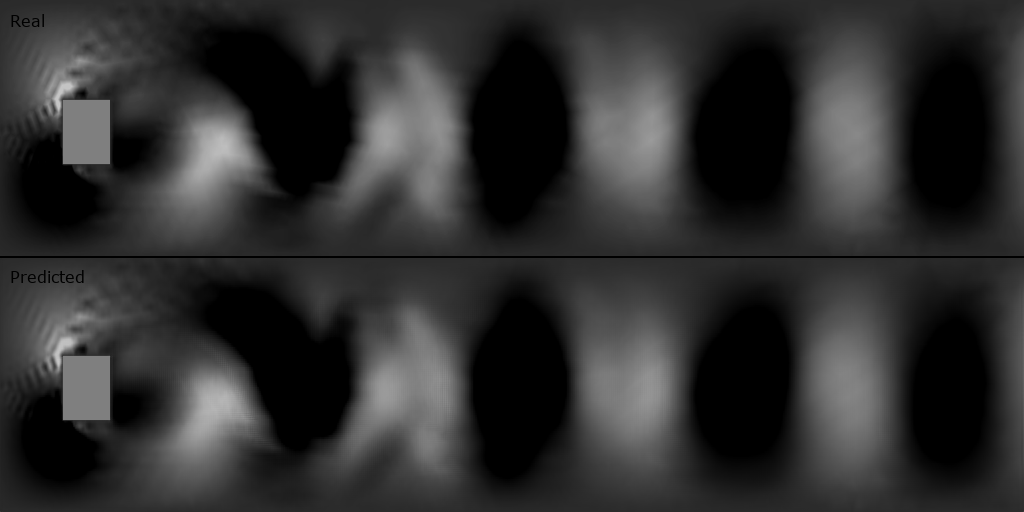
\includegraphics[width=1\linewidth]{imgs/y_recursive_0_speed_8}
  \end{subfigure}

  \begin{subfigure}{.5\textwidth}
    \centering
    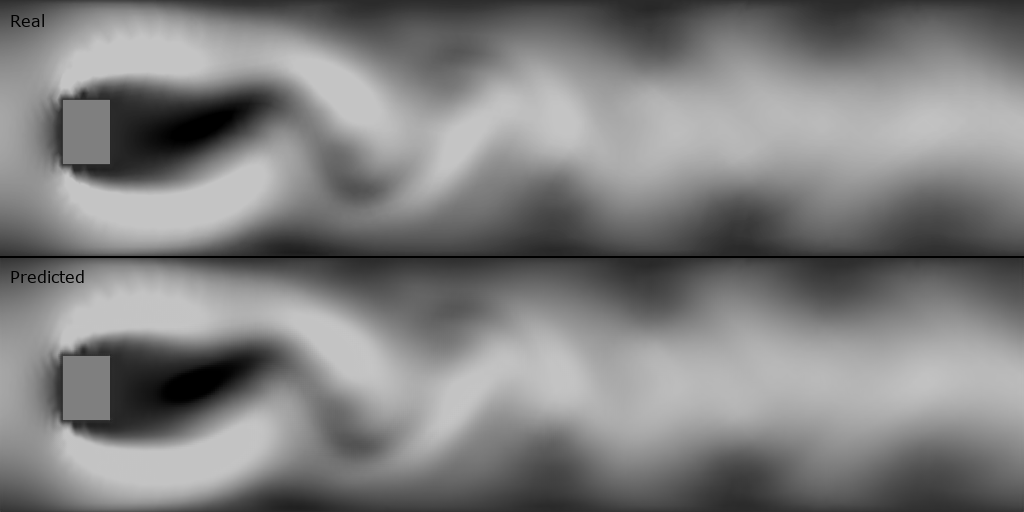
\includegraphics[width=1\linewidth]{imgs/x_recursive_0_speed_39}
  \end{subfigure}
  \begin{subfigure}{.5\textwidth}
    \centering
    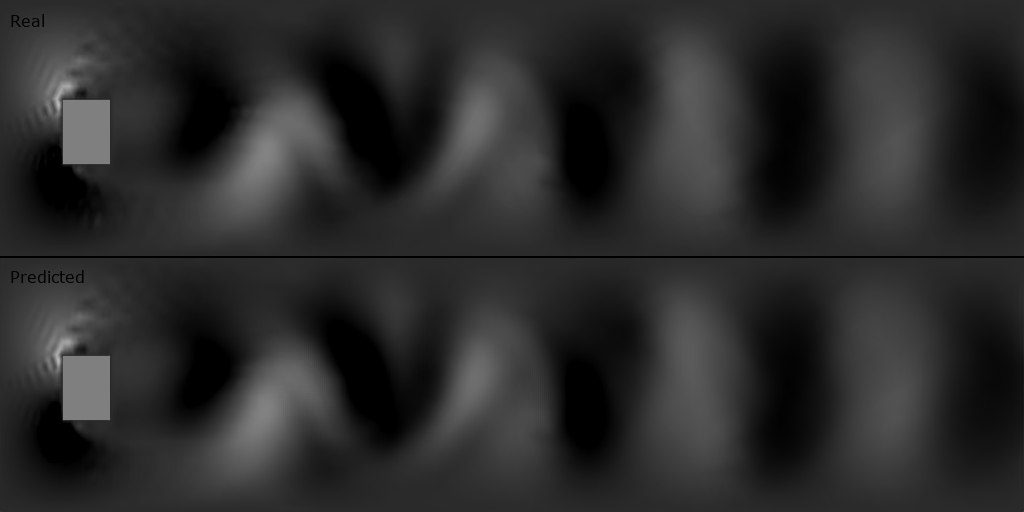
\includegraphics[width=1\linewidth]{imgs/y_recursive_0_speed_39}
  \end{subfigure}
  \begin{center}
    Images form the inflow speed model. The upper two are from simulation with $g=1.9487$ and the lower ones form simulation with $g=3.9358$
  \end{center}

  \begin{subfigure}{.5\textwidth}
    \centering
    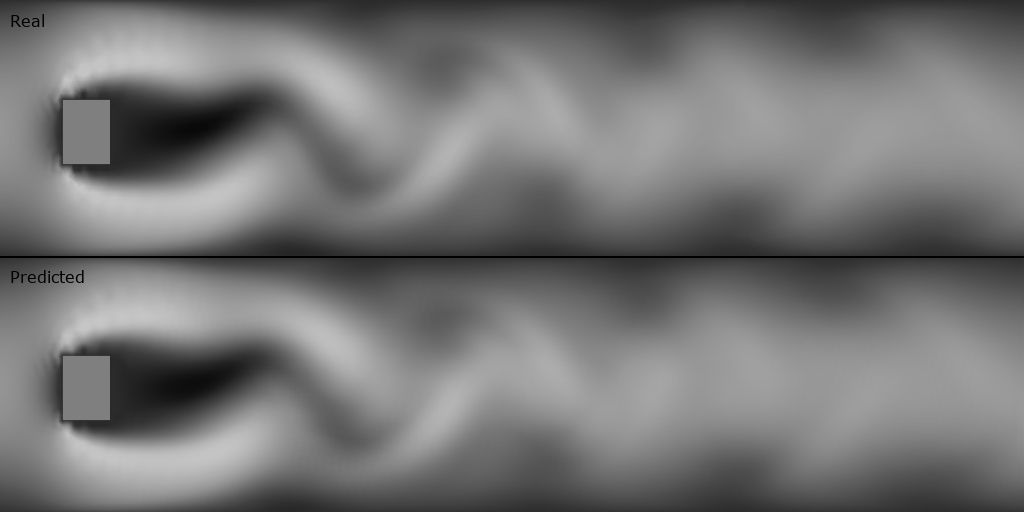
\includegraphics[width=1\linewidth]{imgs/x_recursive_0_fluid_25}
  \end{subfigure}
  \begin{subfigure}{.5\textwidth}
    \centering
    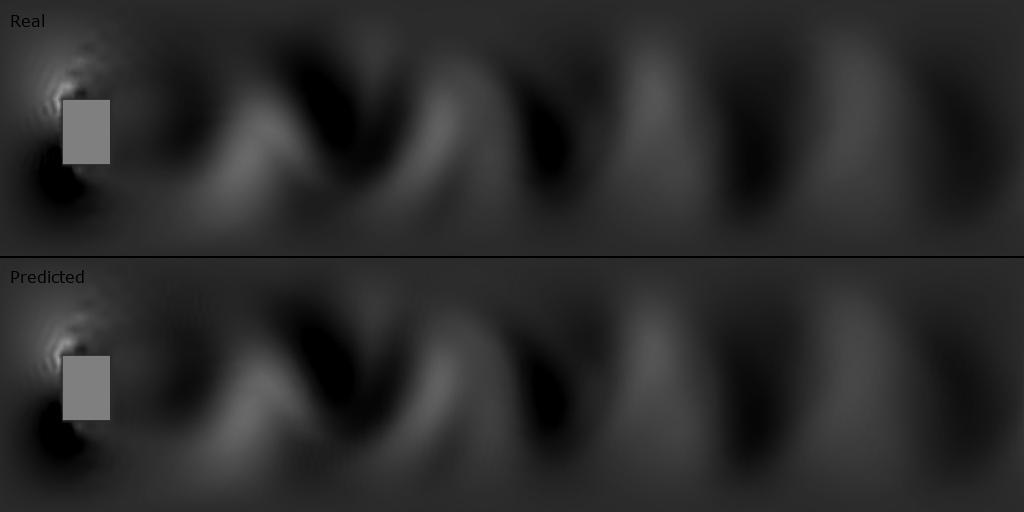
\includegraphics[width=1\linewidth]{imgs/y_recursive_0_fluid_25}
  \end{subfigure}

  \begin{subfigure}{.5\textwidth}
    \centering
    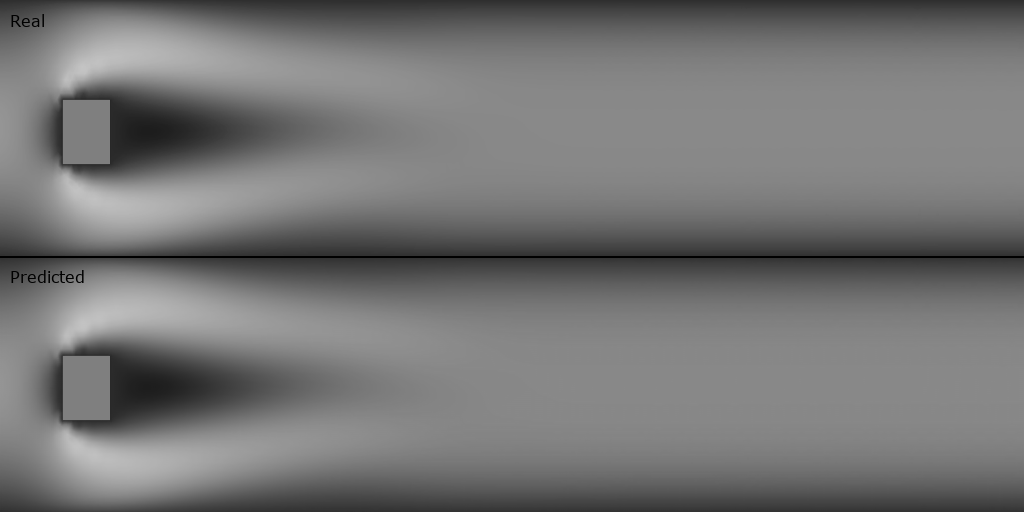
\includegraphics[width=1\linewidth]{imgs/x_recursive_0_fluid_300}
  \end{subfigure}
  \begin{subfigure}{.5\textwidth}
    \centering
    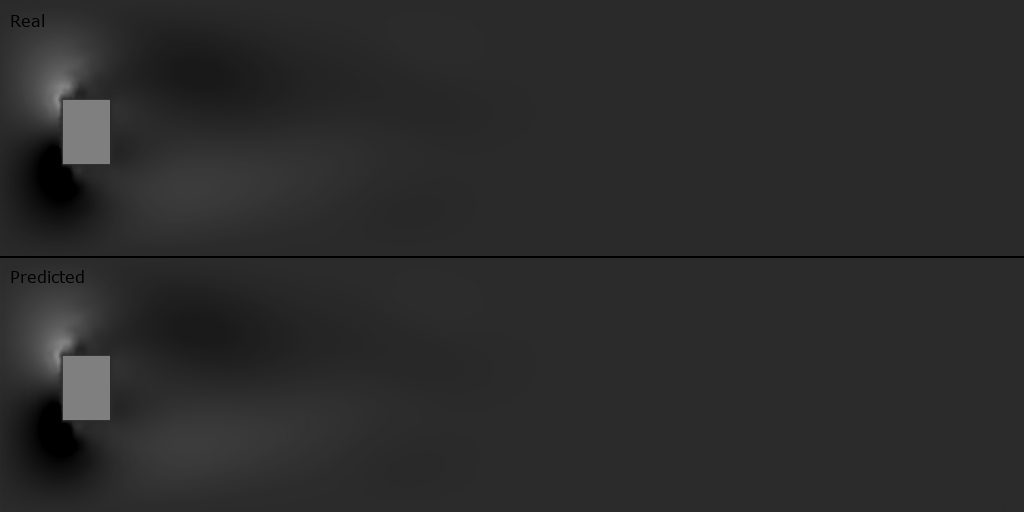
\includegraphics[width=1\linewidth]{imgs/y_recursive_0_fluid_300}
  \end{subfigure}
  \begin{center}
  Images form the viscosity-density model. The upper two are from simulation with $\rho=4.1764, \nu=0.001023$ and the lower ones form simulation with $\rho=4.1764, \nu=0.001023$.
  \end{center}

  \caption{Each image haw tow halves and the upper one shows the ground truth simulation frame. The lower half is the prediction of the model. In the left column, the images are from the x-velocity fie4ld of the simulation and in the right --- form the y-velocity field.}\label{fig:single_images}
\end{figure}

\noindent\textbf{Recursive Application Performance:}
With this evaluation case, we want to see how our models handle recursive application. That is, the output of the network is used again as an input for the prediction of the next simulation frame.

For each recursive evaluation, we generate 40 frames of the corresponding simulation. We did not in any was post-processed the output of the networks before feeding it as an input. We calculate the discussed metrics for each of the predicted frames while comparing them to the corresponding real one.

In our experiments, we performed several recursive evaluations for each simulation while starting at frames with different indexes. We wanted to see how a different starting point in the simulation can affect the frames predicted by the models.

The viscosity-density and inflow speed models are evaluated with several simulations with different parameters. As it is impractical to give the results of the evaluation of each simulation, here we present only several of them. The showed results, however, are representative of the general performance of our models. For this section, we also limit ourselves only to models that do use the pressure field of the simulations. All of the given plots show the mean results for each frame across the evaluations of several models that differ only in the used seed during training. We also plot the standard divination across the evaluations.

The constant model is evaluated with a single simulation --- the one it was trained with.~\reffig{fig:rec_const_psnr} presents the results of the recursive application. During the evaluation, we noticed that the models can more accurately predict the images when the starting frame is further in the simulation. That is, its index relative to the first frame of the simulation is higher. The plots for the constant model in~\reffig{fig:rec_const_psnr} illustrate this.

For the inflow speed model, we present the results from two different simulations in~\reffig{fig:rec_speed_psnr}. We can see the same trend that predicting frames with smaller index is harder. We, however, like to note that the networks appear to be handling the parameters properly and adjust the predicted frames accordingly.\reffig{fig:rec_fluid_psnr} presents two simulations of the viscosity-density model.


\begin{figure}[H]
  \vspace*{-4cm}
  \begin{subfigure}{.5\textwidth}
    \centering
    \includegraphics[width=1\linewidth]{imgs/charts/constant_i10}
  \end{subfigure}
  \begin{subfigure}{.5\textwidth}
    \centering
    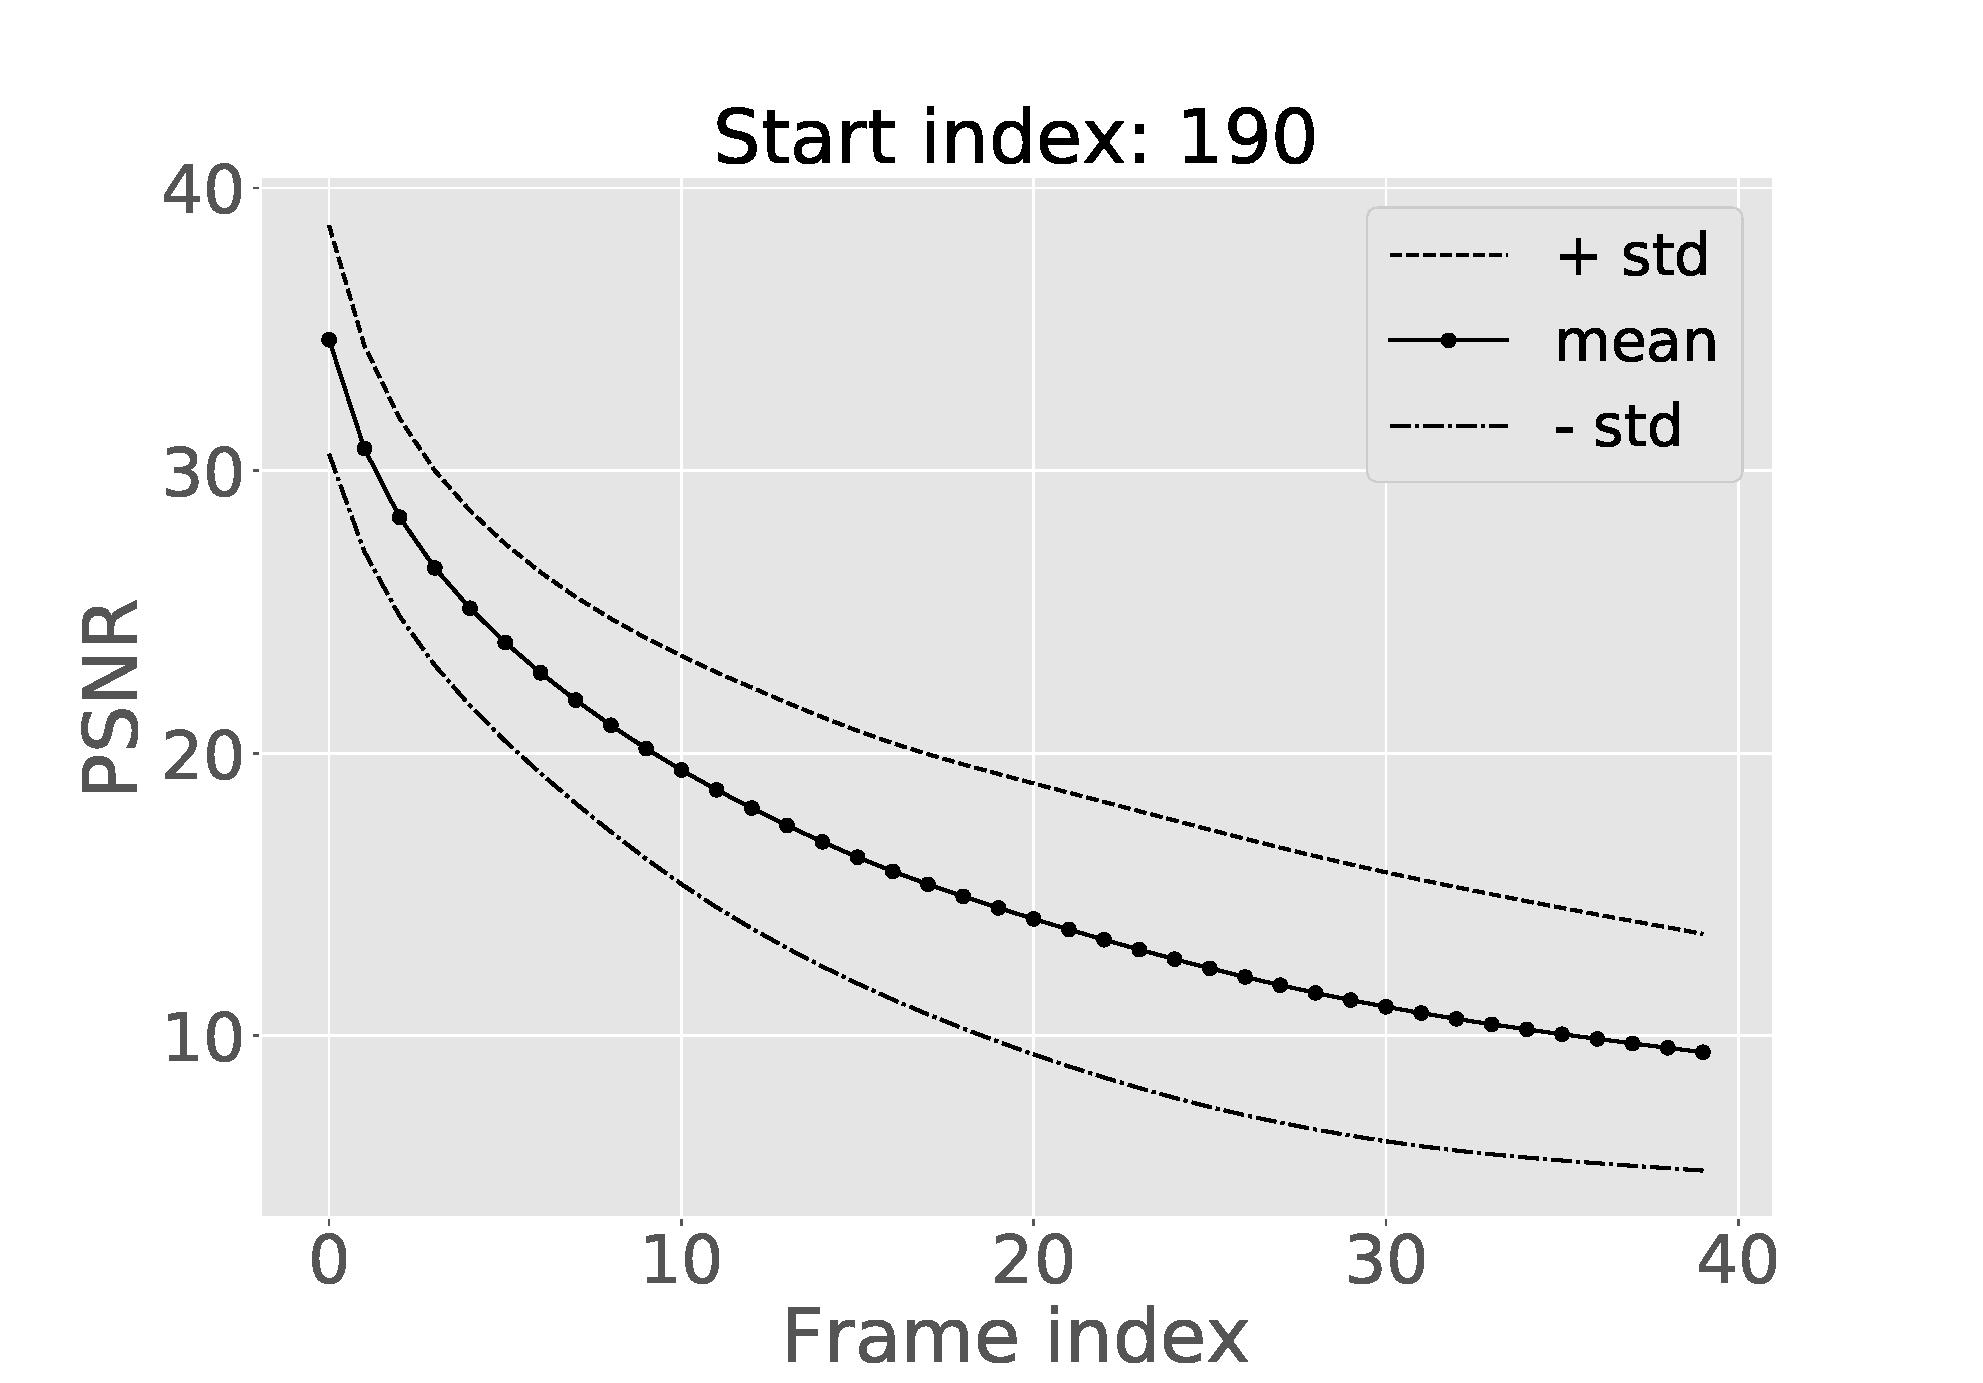
\includegraphics[width=1\linewidth]{imgs/charts/constant_i190}
  \end{subfigure}  
  \caption{The simulation that starts at the 10.\@ frame exhibits unintuitive results. This happens because the PSNR is based on MSE and it can go up if the network produces a homogeneous black image. In this case the PSNR can get higher in the second of the predicted frames. This, however, does not meant that the visual fidelity of the frames is good.}\label{fig:rec_const_psnr}
\end{figure}
\vspace*{-1cm}
\begin{figure}[H]
  \begin{subfigure}{.5\textwidth}
    \centering
    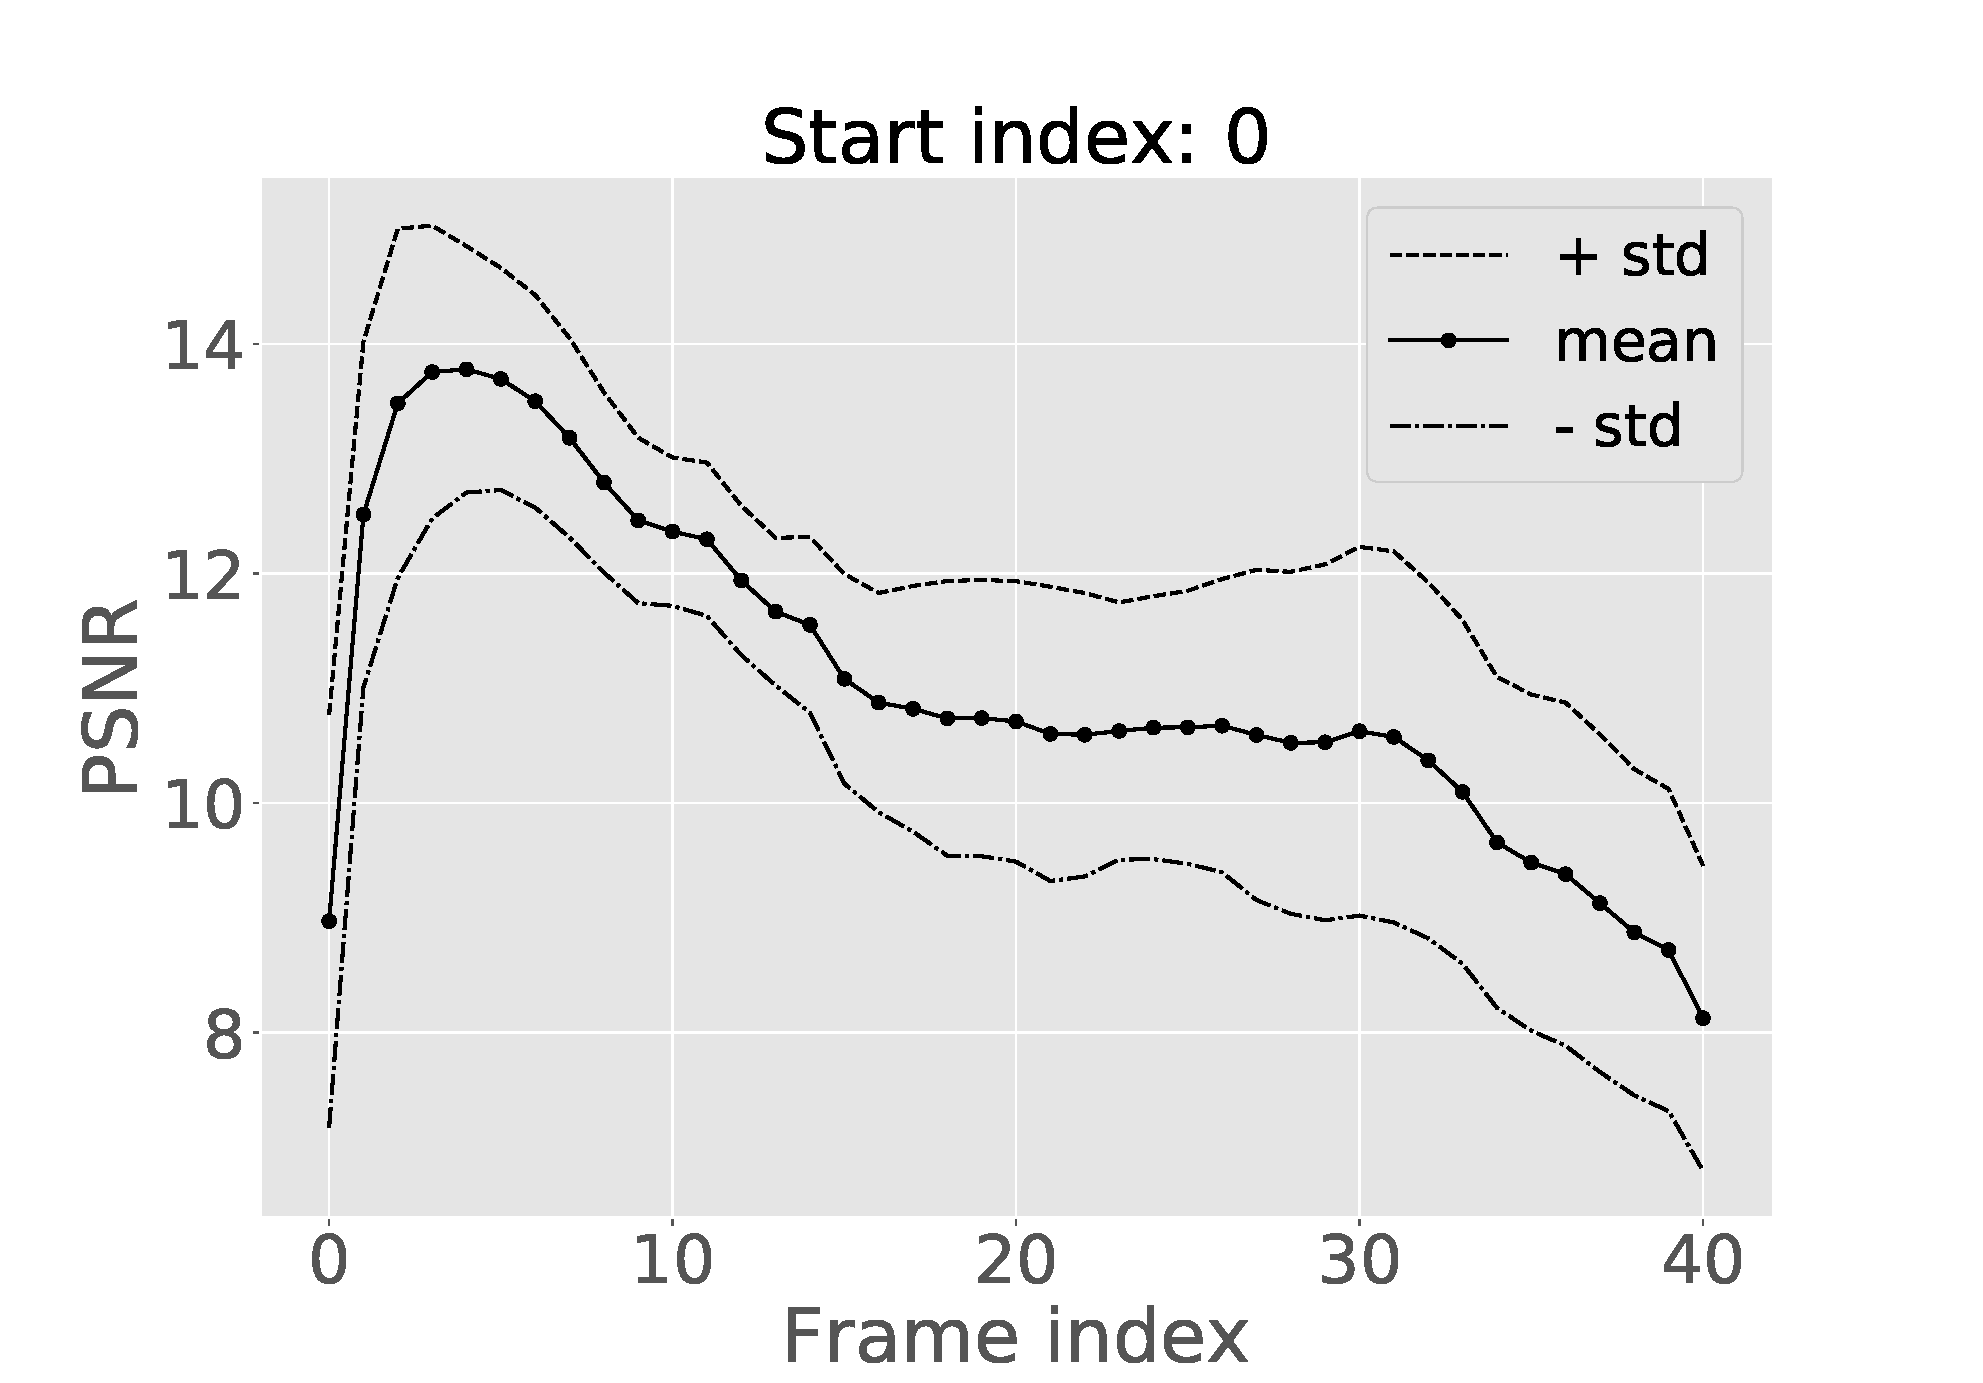
\includegraphics[width=1\linewidth]{imgs/charts/inflow_i10}
  \end{subfigure}
  \begin{subfigure}{.5\textwidth}
    \centering
    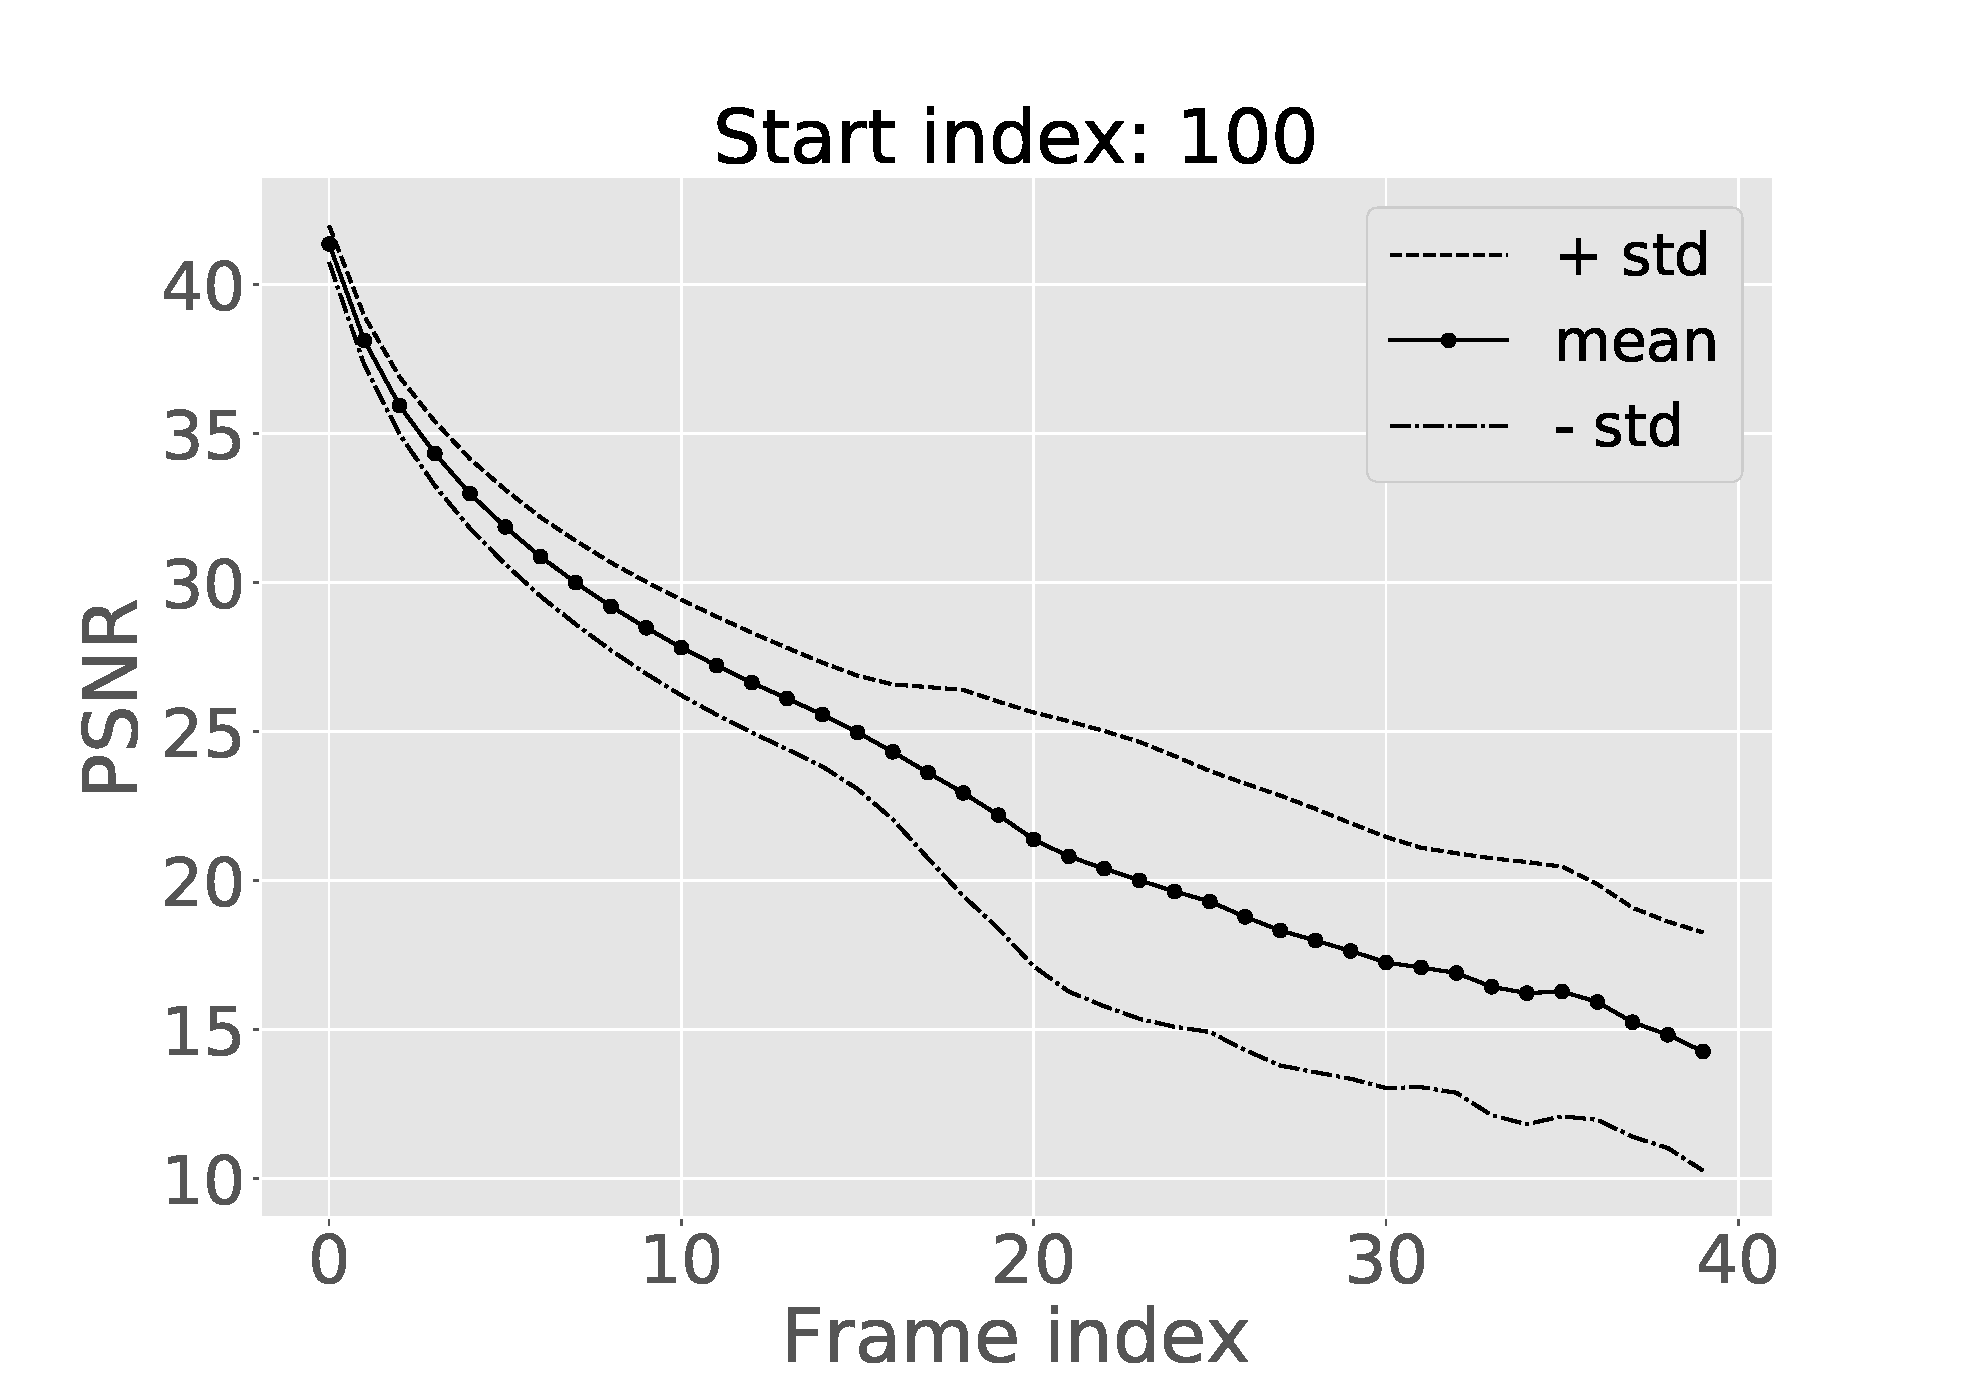
\includegraphics[width=1\linewidth]{imgs/charts/inflow_i1436}
  \end{subfigure}
  \begin{center}
    Recursive evaluations of the inflow speed model on simulation with $g=1.5$. To note is that this simulations was part of the training set. This can explain why the PSNR drops slightly faster on the next charts when it comes to the simulation starting at the 120. \@frame.
  \end{center}
  \begin{subfigure}{.5\textwidth}
    \centering
    \includegraphics[width=1\linewidth]{imgs/charts/inflow_39_s0}
  \end{subfigure}
  \begin{subfigure}{.5\textwidth}
    \centering
    \includegraphics[width=1\linewidth]{imgs/charts/inflow_39_s120}
  \end{subfigure}
  \begin{center}
    Recursive evaluations of the inflow speed model on simulation with $g=3.9358$.
  \end{center}
  \caption{In the evaluations of the inflow speed models, we consistently saw the same behavior as in the constant models. The simulations that at are started at a frame with smaller index are of a lower quality.}\label{fig:rec_speed_psnr}
\end{figure}
\vspace*{-1cm}
\begin{figure}[H]
  \begin{subfigure}{.5\textwidth}
    \centering
    \includegraphics[width=1\linewidth]{imgs/charts/fluid_25_s0}
  \end{subfigure}
  \begin{subfigure}{.5\textwidth}
    \centering
    \includegraphics[width=1\linewidth]{imgs/charts/fluid_25_s120}
  \end{subfigure}
  \begin{center}
    Recursive evaluations of the viscosity-density model on simulation with $\rho=4.1764$ and $\nu=0.001023$.
  \end{center}
  \begin{subfigure}{.5\textwidth}
    \centering
    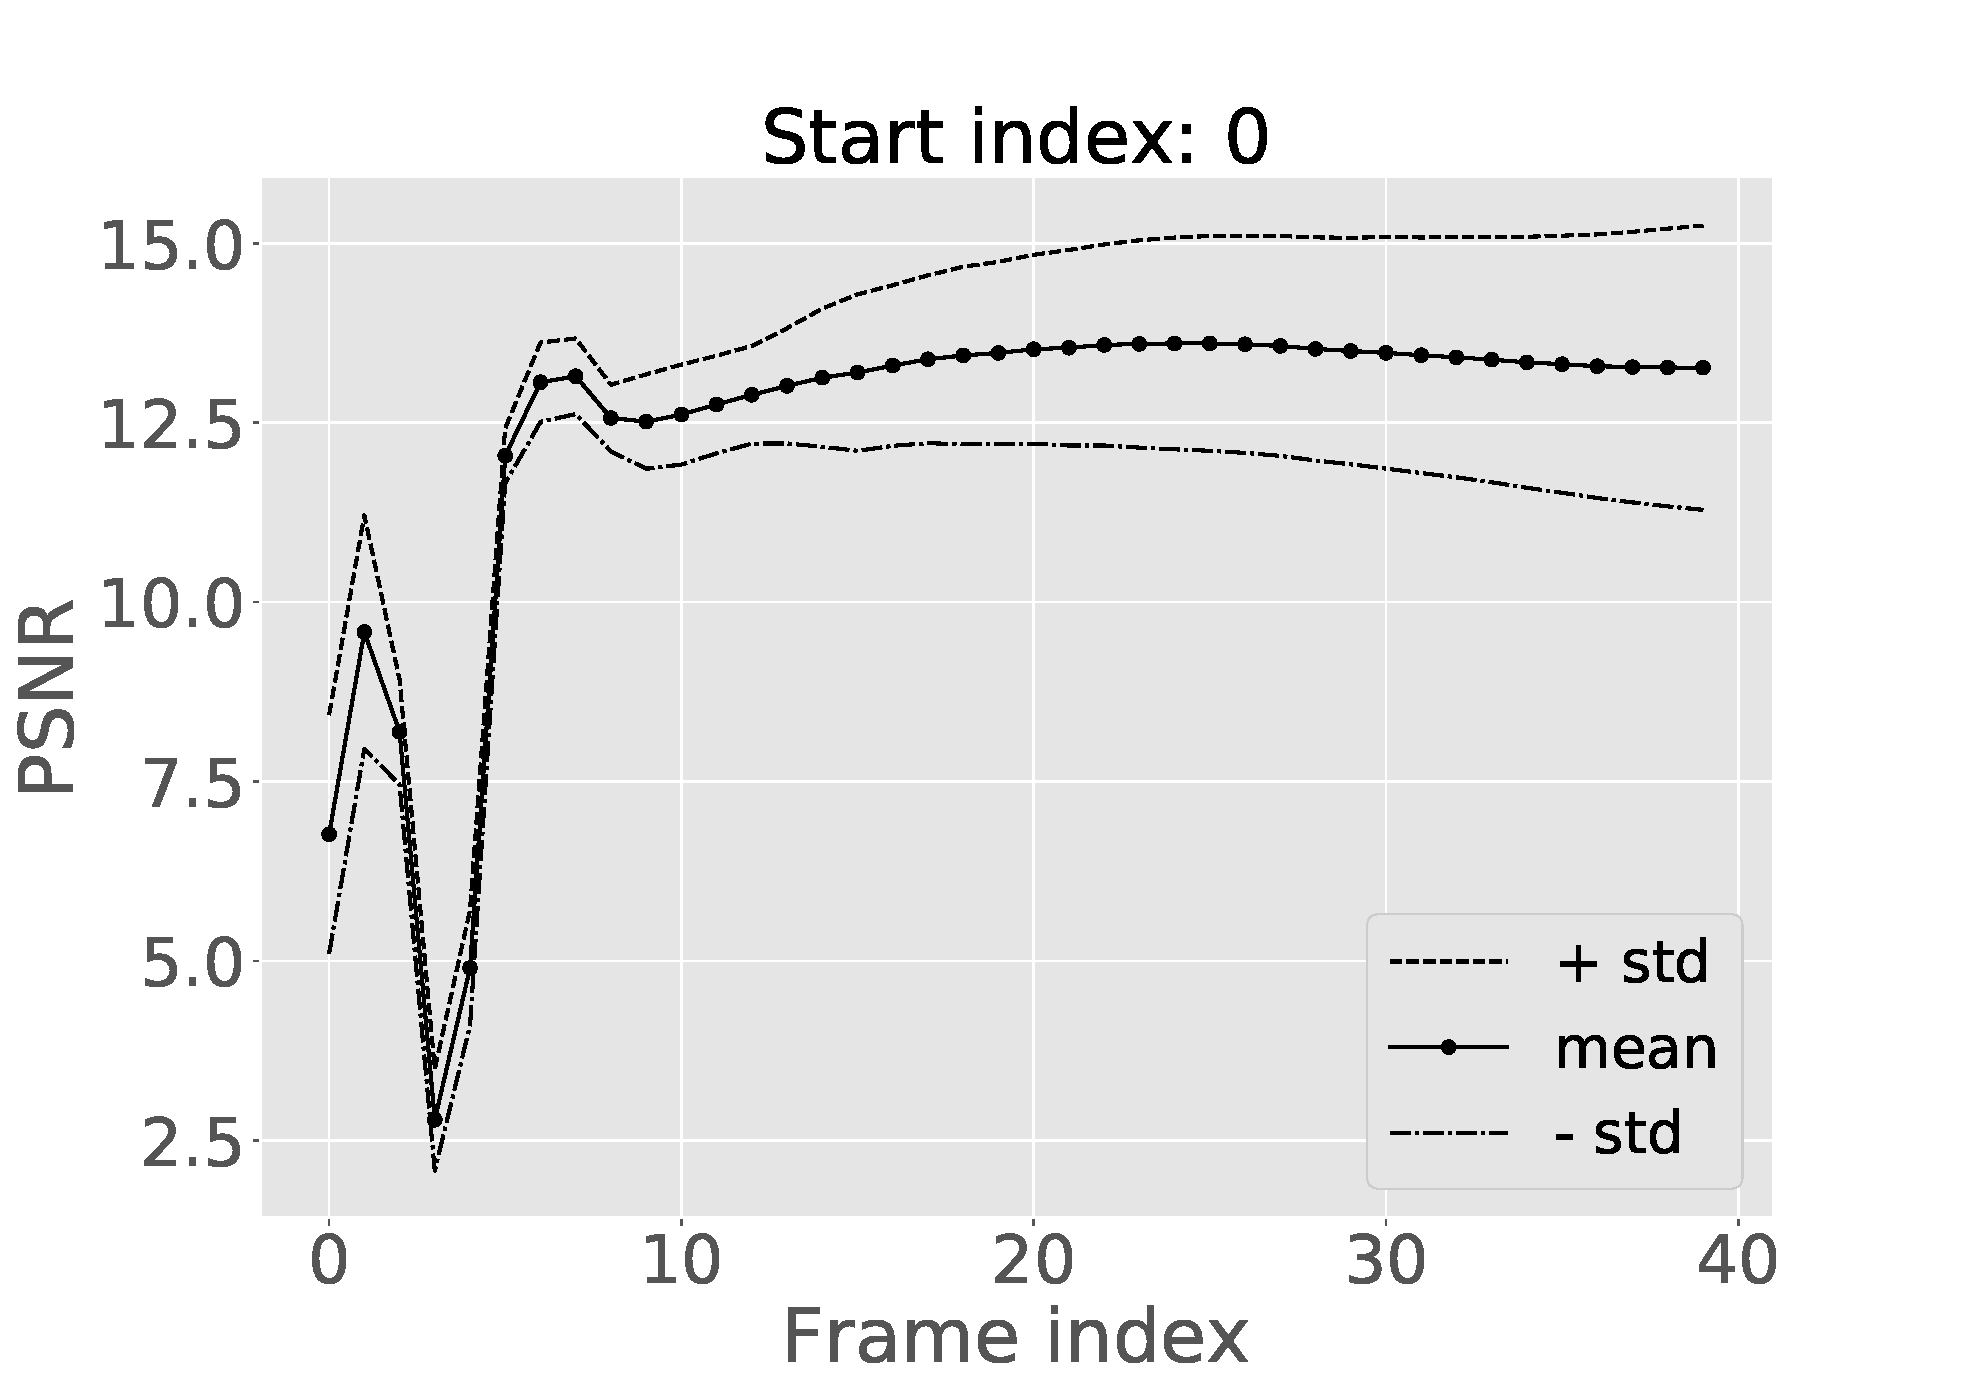
\includegraphics[width=1\linewidth]{imgs/charts/fluid_100_s0}
  \end{subfigure}
  \begin{subfigure}{.5\textwidth}
    \centering
    \includegraphics[width=1\linewidth]{imgs/charts/fluid_100_s120}
  \end{subfigure}
  \begin{center}
    Recursive evaluations of the viscosity-density model on simulation with $\rho=5.7647$ and $\nu=0.001517$.
  \end{center}
  \begin{subfigure}{.5\textwidth}
    \centering
    \includegraphics[width=1\linewidth]{imgs/charts/fluid_300_s0}
  \end{subfigure}
  \begin{subfigure}{.5\textwidth}
    \centering
    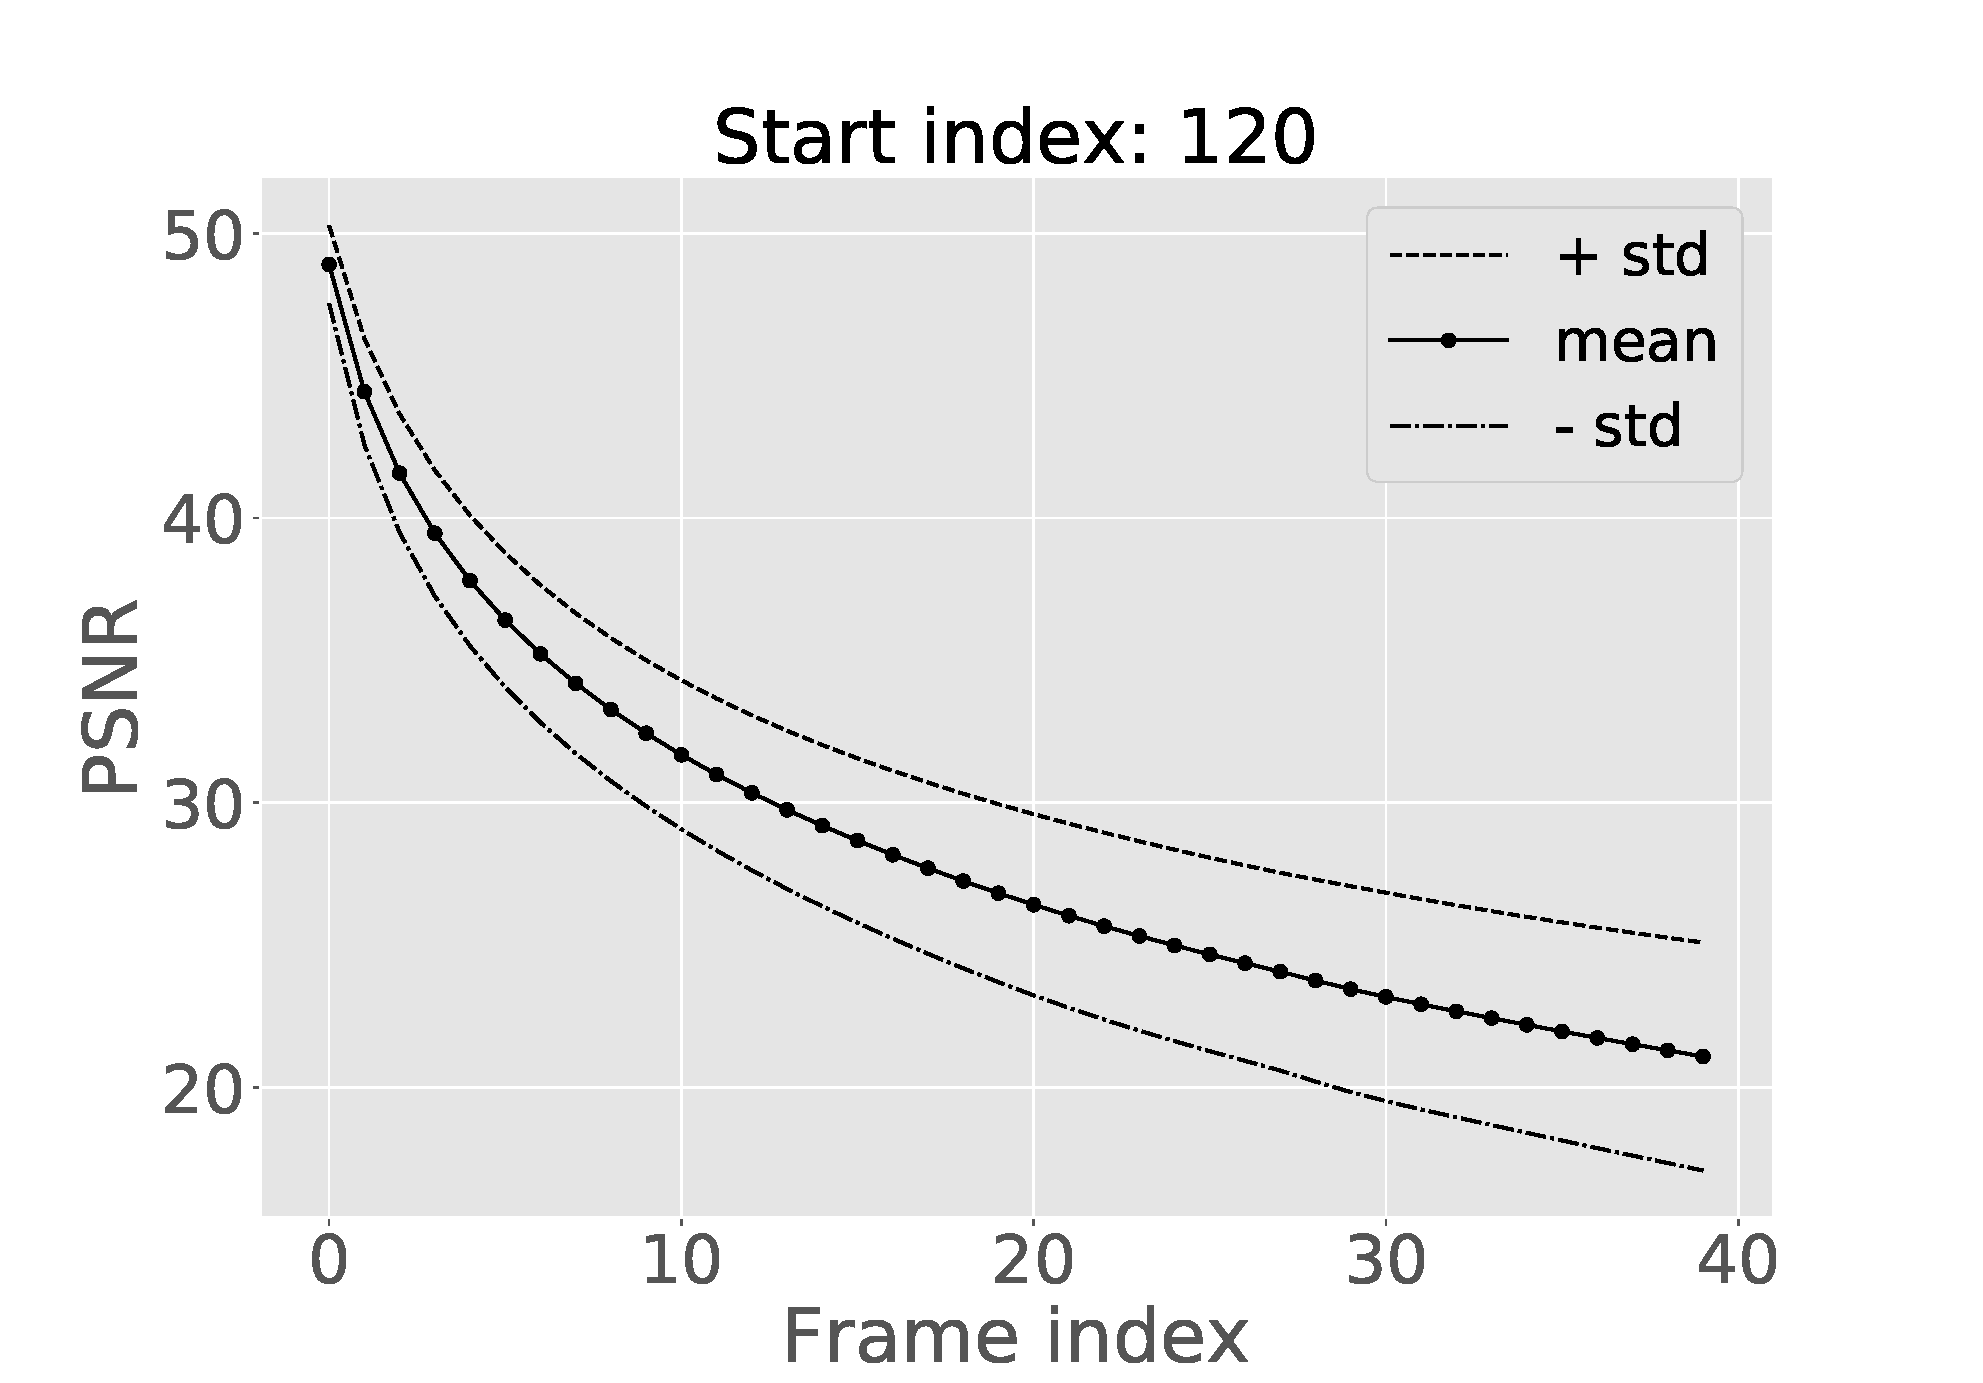
\includegraphics[width=1\linewidth]{imgs/charts/fluid_300_s120}
  \end{subfigure}
  \begin{center}
    Recursive evaluations of the viscosity-density model on simulation with $\rho=6.8235$ and $\nu=0.002876$.
  \end{center}  
  \caption{All of the simulations for the charts are from the test set of the viscosity-density model. The evaluations with starting frame of 0 are consistent with the results from the other models. The evaluations starting at frame 120 are, however, much more stable as indicated by the standard deviation. We again attribute that to the over all stability of the model due to the large amount of train data used to train the models of this type.}\label{fig:rec_fluid_psnr}
\end{figure}

We noticed that across all model types, for some of the predicted frames, certain visual artifacts can occur. In some cases, those are in the form of a pattern that spans across the image. This pattern seems to be recognized by the models as not part of the flow and does not disrupt the structure of the flow. Other artifacts, however, can look much more like features of the fluid flow. In this case, the network will develop them as it develops the real flow. These artifacts accumulate with each predicted frame and become apparent after around the 10.\@ frame. In our experiments, we managed to minimize the artifacts by making the networks bigger but we never could mitigate them completely.

We again do not explicitly give the correlation between the predicted and real frames. In all cases, the correlation stayed very close to $1$ and varied in the range $[0.98, 0.99998]$. The difference-metrics are summarized in~\reftab{tab:recursive_inflow} and~\reftab{tab:recursive_fluid}.

\begin{table}[H]
  \begin{center}
    Inflow speed model
  \end{center}
  \begin{center}
    \begin{tabular}{l|cc|cc}
     \textbf{Frame} & \multicolumn{2}{c|} {\shortstack{\textbf{Start index: 120}\\$g=1.9487$}}& \multicolumn{2}{c}{\shortstack{\textbf{Start index: 120}\\$g=3.9358$}}\\
      \hline 
                     &\multicolumn{2}{c|}{} & &\\
                     & {Average difference} & {Max difference}  &  {Average difference} & {Max difference}\\
      \emph{Frame 1}       &34.27(0.02) & 52.72(0.40)    &35.91(0.02) & 51.76(0.38)   \\
      \emph{Frame 5}       &33.86(0.11) & 60.41(1.62)    &35.84(0.10) & 53.13(0.54)   \\
      \emph{Frame 10}      &33.99(0.17) & 66.04(2.16)    &36.01(0.15) & 54.59(1.14)   \\
      \emph{Frame 15}      &33.80(0.20) & 76.40(3.67)    &35.91(0.20) & 58.90(1.97)   \\
      \emph{Frame 20}      &34.27(0.22) & 75.39(3.07)    &35.89(0.24) & 62.60(2.94)   \\
      \emph{Frame 25}      &33.91(0.22) & 83.45(3.06)    &35.93(0.28) & 61.07(2.60)   \\
      \emph{Frame 30}      &34.13(0.24) & 79.15(2.20)    &35.73(0.33) & 66.69(4.21)   \\
      \emph{Frame 35}      &34.38(0.23) & 83.52(2.09)    &35.94(0.35) & 65.55(4.18)   \\      
    \end{tabular}
  \end{center}
  \caption{Again, all of the numbers are in percents and are averaged across the evaluations of models trained only with difference in the used seed. The standard deviation is given in the parenthesis. To note is that the maximum difference is high for almost all frames. This is to be expected from our models as they primarily target the visual quality of the results. The average difference on the other hand stays relatively stable across the frames. Still, average difference of over 30\% unsatisfactory even for coarse simulation.}\label{tab:recursive_inflow}
\end{table}

\begin{table}[H]
  \begin{center}
    Viscosity-density model
  \end{center}
  \begin{center}
    \begin{tabular}{l|cc|cc}
      \textbf{Frame} & \multicolumn{2}{c|} {\shortstack{\textbf{Start index: 120}\\$\rho=4.1764, \nu=0.001023$}}&\multicolumn{2}{c}{\shortstack{\textbf{Start index: 120}\\$\rho=6.8235, \nu=0.002876$}}\\
      \hline 
                     &\multicolumn{2}{c|}{} & &\\
                     & {Average difference} & {Max difference}  &  {Average difference} & {Max difference}\\
      \emph{Frame 1}       &35.87(0.03) & 52.04(0.38)           &35.27(0.00) & 52.16(1.45)   \\
      \emph{Frame 5}       &36.33(0.16) & 54.48(0.89)           &35.27(0.02) & 54.23(3.28)   \\
      \emph{Frame 10}      &35.75(0.24) & 55.87(1.57)           &35.28(0.04) & 54.89(3.31)   \\
      \emph{Frame 15}      &35.77(0.30) & 58.47(2.10)           &35.29(0.06) & 55.67(2.79)   \\
      \emph{Frame 20}      &35.66(0.32) & 59.87(2.54)           &35.30(0.09) & 56.59(2.05)   \\
      \emph{Frame 25}      &35.63(0.37) & 60.86(2.54)           &35.32(0.11) & 57.54(2.48)   \\
      \emph{Frame 30}      &35.64(0.40) & 61.16(3.37)           &35.34(0.13) & 58.30(3.05)   \\
      \emph{Frame 35}      &35.78(0.39) & 63.11(1.57)           &35.36(0.15) & 59.17(3.42)   \\      
    \end{tabular}
  \end{center}
  \caption{For the viscosity-density model the average differences are again stable across the frames of the predicted simulations. The maximum differences grow as the predictions get more inaccurate and more artefacts appear in the predicted frames.}\label{tab:recursive_fluid}
\end{table}

\noindent\textbf{Performance:} All of the models were evaluated on an Nvidia GTX 980Ti GPU.\@In all cases, the forward propagation of a single simulation frame took between 5 and 20 ms (milliseconds). In comparison, during the data generation, HiFlow needed between 1000 and 1500 ms for a single simulation timestep while using 12 MPI processes. This does not include the time needed for rendering the results of the simulation. To note is that this is not a one-to-one comparison as HiFlow runs on the CPU and uses MPI and OpenMP for parallelization. Also, we performed all the real simulations with HiFlow on a Intel Xeon E5-2650 v4 CPU.

We, however, think that the results show the potential of our approach when it comes to performance.

\section{Conclusion}\label{conclusion}
The results presented in this paper suggest that solving a numerical task trough image-to-image translation can be a viable approach. We showed how conditional GANs can be used to learn the image representations of the solutions of a fluid simulation according to the Navier-Stokes equations. We built several models that can generalize different parts of the parameters of the simulations and gave concrete numbers that quantify the results. Even though the accuracy of the results is not high enough for the predicted simulations to be considered ``true'', the visual quality of the images allows a human observer to see the general development of the fluid flow.

We believe that out approach can be extended to other simulation types as well. We see our work as preliminary research and we believe that the method can be further developed and investigated. Strategies for improving the models that were considered but not implemented include:
\begin{itemize}
\item[$\cdot$] using an LSTM~\cite{lstm} layer in the networks --- our models have the limitation that during training they don't know about the artifact on the images caused by themselves. We think an LSTM layer can mitigate this problem.
\item[$\cdot$] preprocessing the input for and postprocessing the output of the networks --- morphological operations like opening and closing can also be used to minimize the artifacts in the predicted frames.
\item[$\cdot$] further investigation of the effects of using RGB-images instead of grayscale ones.
\end{itemize}
\begin{figure}[H]
  \vspace*{-4.5cm}
  \begin{subfigure}{.5\textwidth}
    \centering
    \large{x-velocity}
    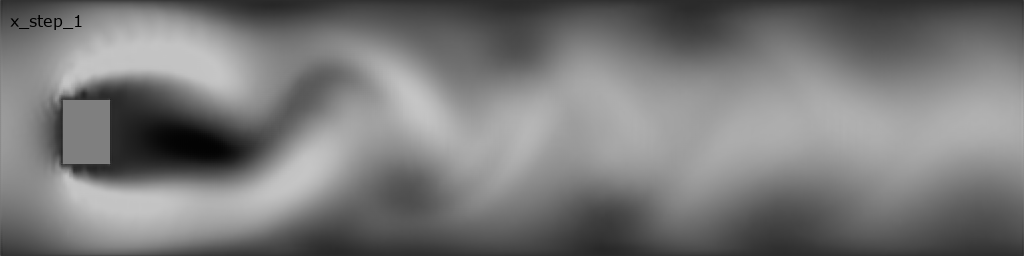
\includegraphics[width=1\linewidth]{imgs/sims/constant/x_step_1}
  \end{subfigure}
  \begin{subfigure}{.5\textwidth}
    \centering
    \large{y-velocity}
    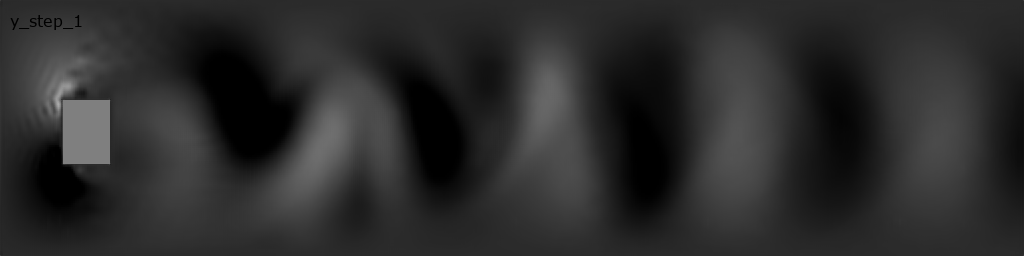
\includegraphics[width=1\linewidth]{imgs/sims/constant/y_step_1}
  \end{subfigure}

  \begin{subfigure}{.5\textwidth}
    \centering
    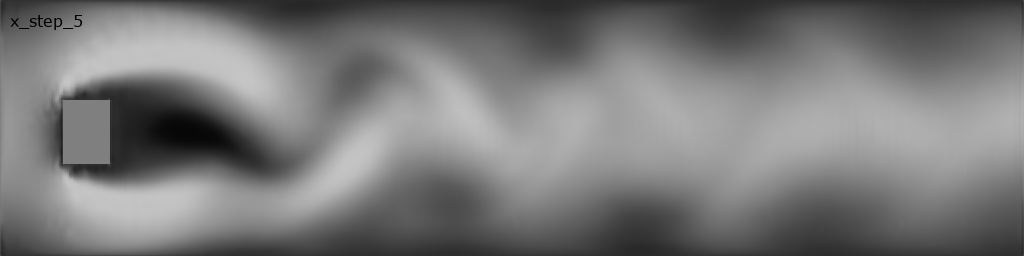
\includegraphics[width=1\linewidth]{imgs/sims/constant/x_step_5}
  \end{subfigure}
  \begin{subfigure}{.5\textwidth}
    \centering
    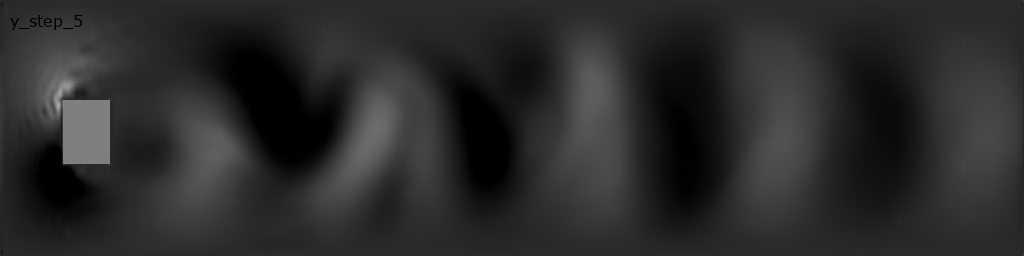
\includegraphics[width=1\linewidth]{imgs/sims/constant/y_step_5}
  \end{subfigure}

  \begin{subfigure}{.5\textwidth}
    \centering
    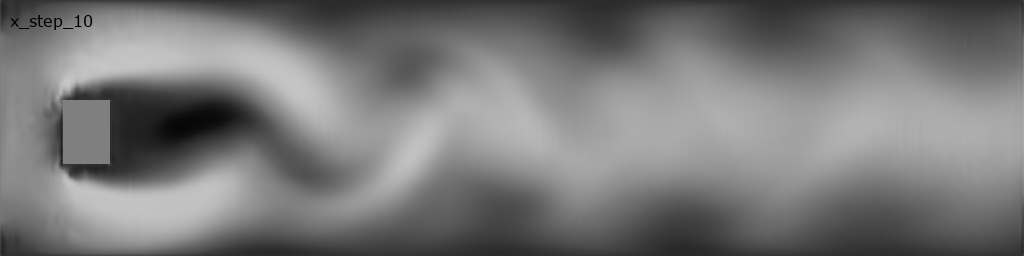
\includegraphics[width=1\linewidth]{imgs/sims/constant/x_step_10}
  \end{subfigure}
  \begin{subfigure}{.5\textwidth}
    \centering
    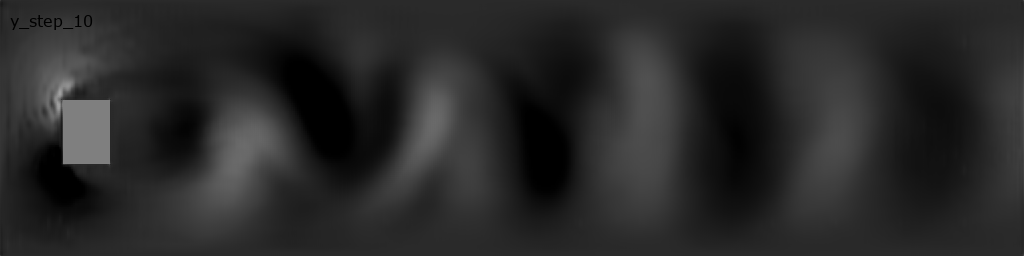
\includegraphics[width=1\linewidth]{imgs/sims/constant/y_step_10}
  \end{subfigure}

  \begin{subfigure}{.5\textwidth}
    \centering
    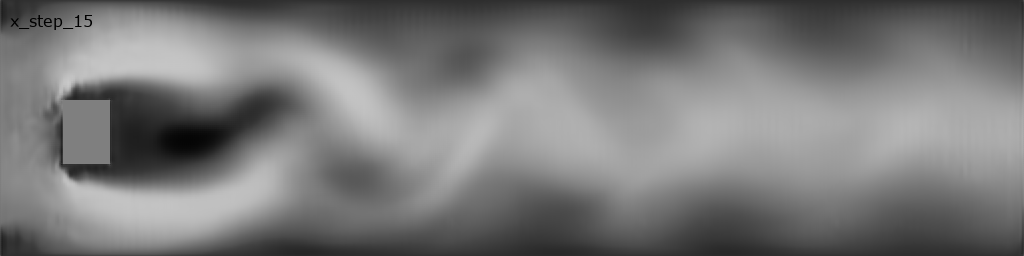
\includegraphics[width=1\linewidth]{imgs/sims/constant/x_step_15}
  \end{subfigure}
  \begin{subfigure}{.5\textwidth}
    \centering
    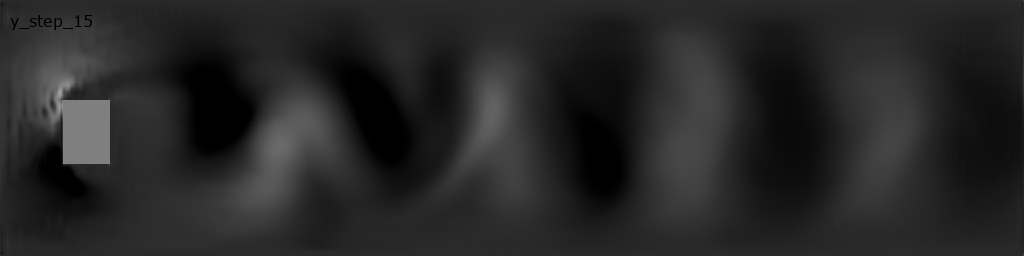
\includegraphics[width=1\linewidth]{imgs/sims/constant/y_step_15}
  \end{subfigure}

  \begin{subfigure}{.5\textwidth}
    \centering
    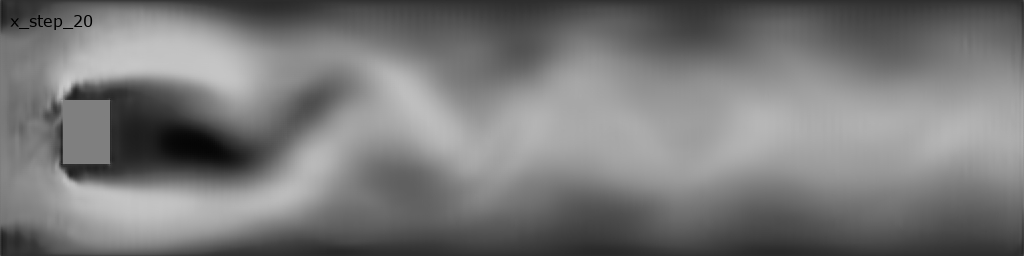
\includegraphics[width=1\linewidth]{imgs/sims/constant/x_step_20}
  \end{subfigure}
  \begin{subfigure}{.5\textwidth}
    \centering
    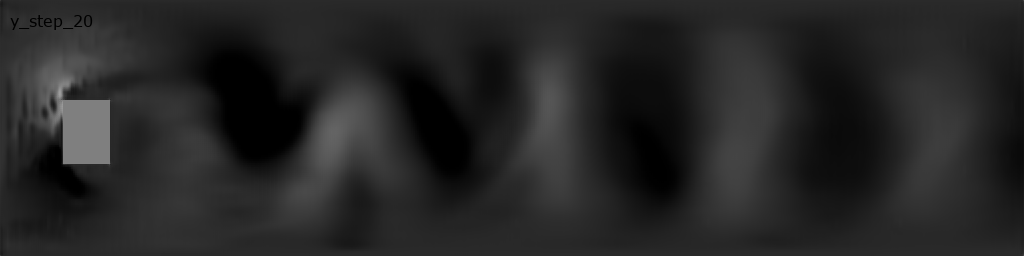
\includegraphics[width=1\linewidth]{imgs/sims/constant/y_step_20}
  \end{subfigure}

  \begin{subfigure}{.5\textwidth}
    \centering
    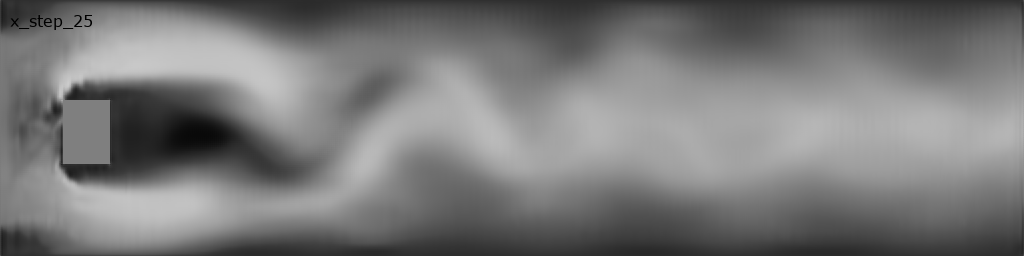
\includegraphics[width=1\linewidth]{imgs/sims/constant/x_step_25}
  \end{subfigure}
  \begin{subfigure}{.5\textwidth}
    \centering
    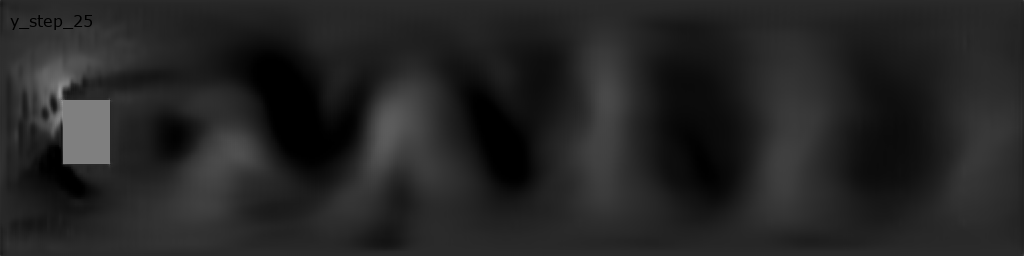
\includegraphics[width=1\linewidth]{imgs/sims/constant/y_step_25}
  \end{subfigure}

  \caption{These frames are generated by the constant model. The artifacts become apparent after the 10.\@ one.}\label{fig:const_sim}
\end{figure}
\vspace*{-1cm}
\begin{figure}[H]
  \begin{subfigure}{.5\textwidth}
    \centering
    \large{x-velocity}
    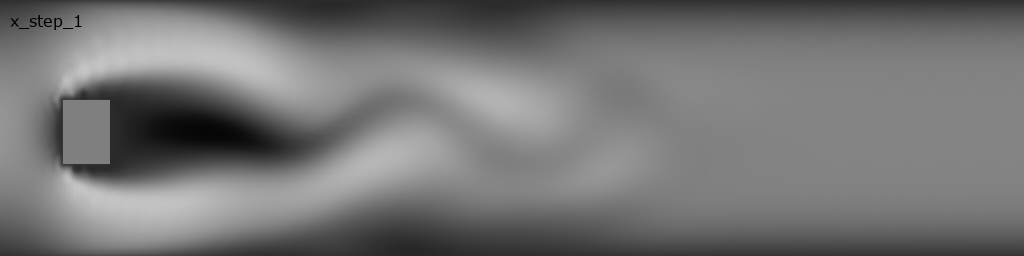
\includegraphics[width=1\linewidth]{imgs/sims/fluid/x_step_1}
  \end{subfigure}
  \begin{subfigure}{.5\textwidth}
    \centering
    \large{y-velocity}
    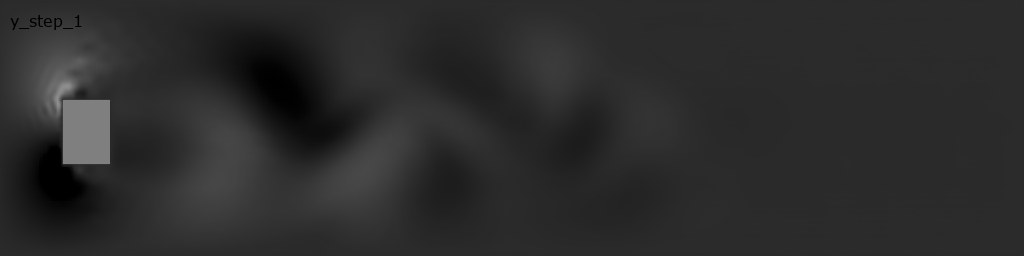
\includegraphics[width=1\linewidth]{imgs/sims/fluid/y_step_1}
  \end{subfigure}

  \begin{subfigure}{.5\textwidth}
    \centering
    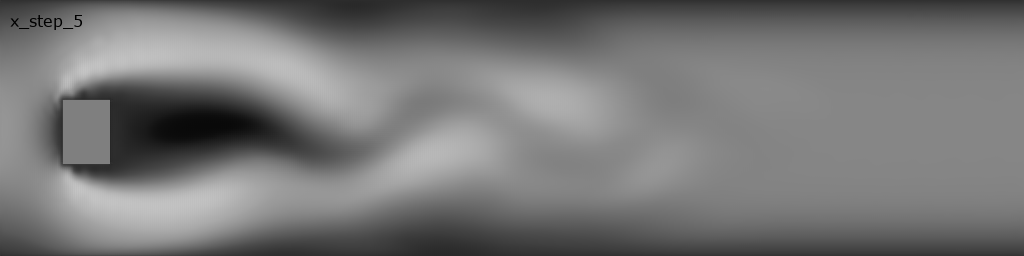
\includegraphics[width=1\linewidth]{imgs/sims/fluid/x_step_5}
  \end{subfigure}
  \begin{subfigure}{.5\textwidth}
    \centering
    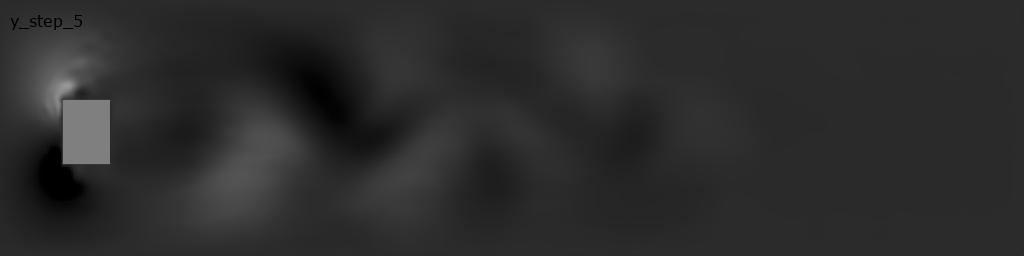
\includegraphics[width=1\linewidth]{imgs/sims/fluid/y_step_5}
  \end{subfigure}

  \begin{subfigure}{.5\textwidth}
    \centering
    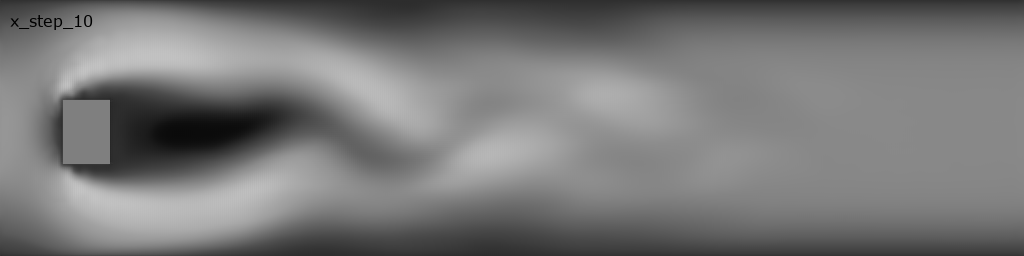
\includegraphics[width=1\linewidth]{imgs/sims/fluid/x_step_10}
  \end{subfigure}
  \begin{subfigure}{.5\textwidth}
    \centering
    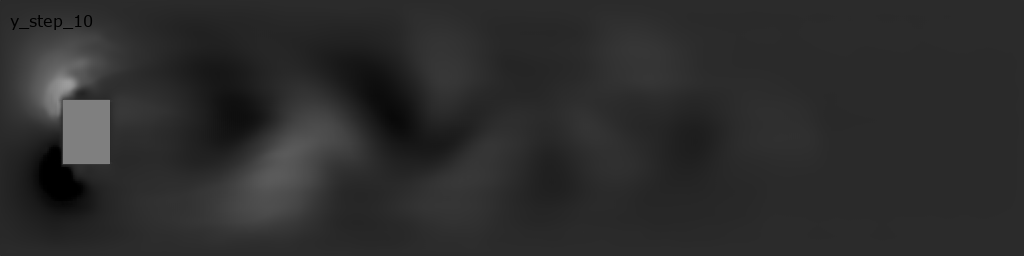
\includegraphics[width=1\linewidth]{imgs/sims/fluid/y_step_10}
  \end{subfigure}

  \begin{subfigure}{.5\textwidth}
    \centering
    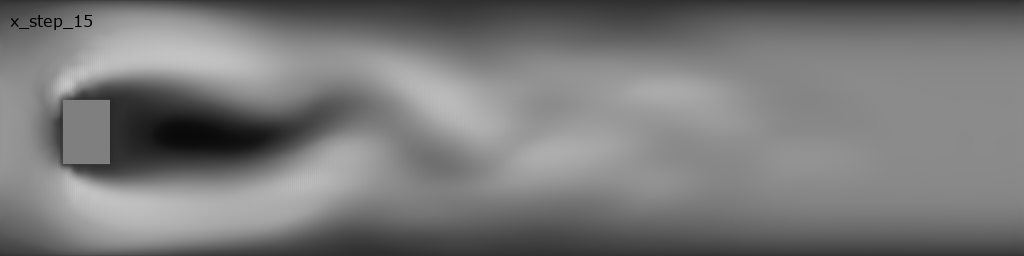
\includegraphics[width=1\linewidth]{imgs/sims/fluid/x_step_15}
  \end{subfigure}
  \begin{subfigure}{.5\textwidth}
    \centering
    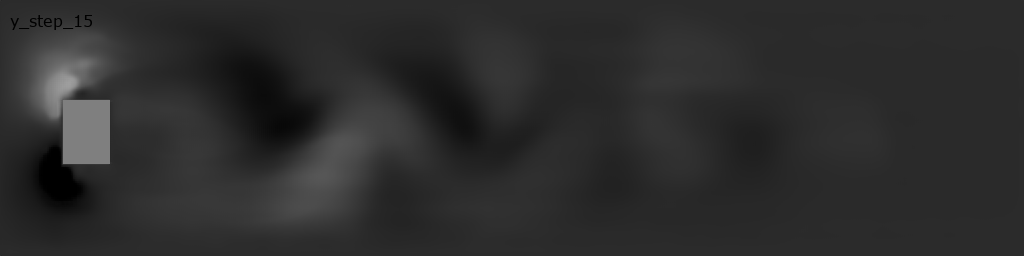
\includegraphics[width=1\linewidth]{imgs/sims/fluid/y_step_15}
  \end{subfigure}


  \begin{subfigure}{.5\textwidth}
    \centering
    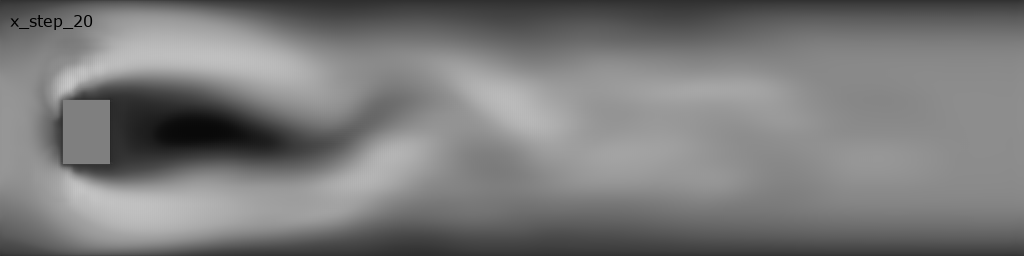
\includegraphics[width=1\linewidth]{imgs/sims/fluid/x_step_20}
  \end{subfigure}
  \begin{subfigure}{.5\textwidth}
    \centering
    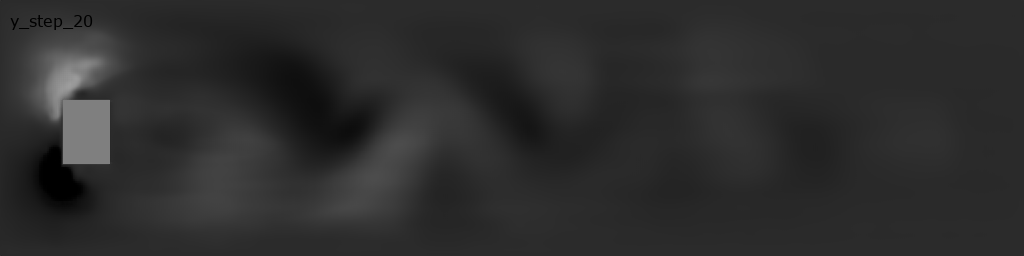
\includegraphics[width=1\linewidth]{imgs/sims/fluid/y_step_20}
  \end{subfigure}

  \begin{subfigure}{.5\textwidth}
    \centering
    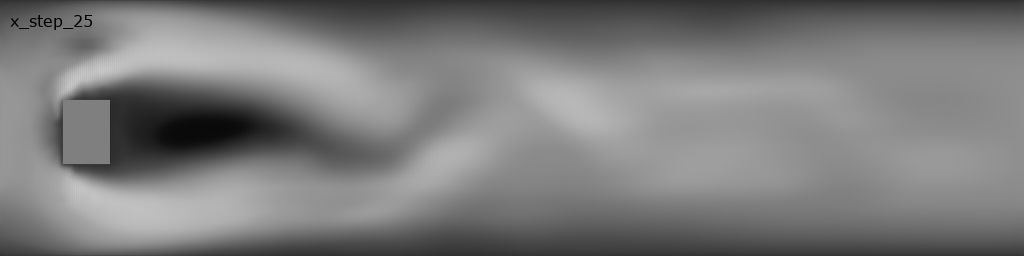
\includegraphics[width=1\linewidth]{imgs/sims/fluid/x_step_25}
  \end{subfigure}
  \begin{subfigure}{.5\textwidth}
    \centering
    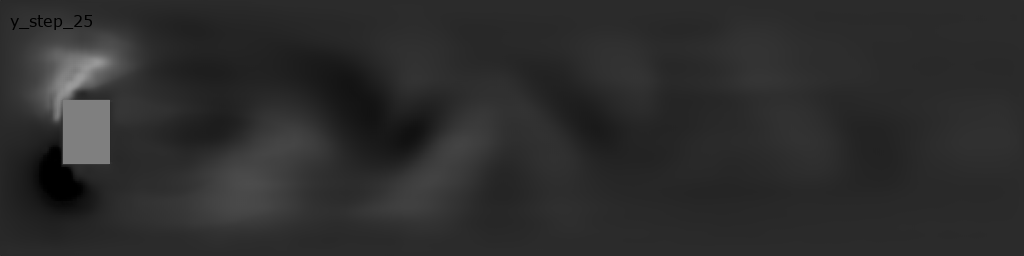
\includegraphics[width=1\linewidth]{imgs/sims/fluid/y_step_25}
  \end{subfigure}

  \caption{Example frames generated by the viscosity-density model. The parameters for this particular simulation are $\nu=4.17647, \rho = 0.001, g=1.4$}\label{fig:fluid_sim}
\end{figure}
\clearpage
\bibliographystyle{splncs04}
\bibliography{egbib}

\begin{subappendices}
\renewcommand{\thesection}{\Alph{section}}%

\section{Networks architectures and hyperparameters}\label{app1}
\emph{Here we give the exact details on the architectures of the used networks.} The code for all of the models and experiments can be found at \url{https://github.com/palikar/flow_predict}.

The architectures are almost entirely based on~\cite{pix2pix} and~\cite{radford2015}. Both the generator and the discriminator networks are comprised of two types of blocks of layers. We will denote a Convolution-BatchNorm-ReLU block with $k$ filters with $Ck$ and Convolution-BatchNorm-Dropout-ReLU with $k$ filters $CDk$. The dropout rate for each dropout layer is 50\%. All convolutions use $4\times4$ filters applied with a stride of $2$.

\noindent\textbf{Generator Architecture:}
The generator is an follows the encoder-decoder principle. All model types use 6 layer encoder and decoder. The model types differ only in the number of filters that they have in the blocks. As we use the U-Net architecture, there are also skip connections between each block $i$ in the encoder and the block $n-i$ in the decoder where $n$ is the total number of blocks in the network. The skip connections concatenate the results from both blocks $i$ and $i-i$.

The concrete encoder-decoders for each model type are as follows:
\begin{itemize}
\item[$\cdot$] Constant model:\newline
  \emph{Encoder}: \texttt{C32-C64-C128-C256-C256-C256}\newline
  \emph{Decoder}: \texttt{CD256-C512-C512-C256-C128-C64}
\item[$\cdot$] Inflow speed model:\newline
  \emph{Encoder}: \texttt{C48-C96-C192-C384-C384-C384}\newline
  \emph{Decoder}: \texttt{CD384-C768-C768-C384-C192-C96}
\item[$\cdot$] Viscosity-Density model:\newline
  \emph{Encoder}: \texttt{C64-C128-C256-C512-C512-C512} \newline
  \emph{Decoder}: \texttt{CD512-C1024-C1024-C512-C256-C128}
\end{itemize}

The ReLUs in the encoders are leaky (slope of $0.2$) and those in the decoders are not. At the end of each decoder, there is also a convolution layer that maps to the final channel count of the output. This final convolution is followed by a $\tanh$-function.

\noindent\textbf{Discriminator Architecture:}
We adopt the $256\times256$ variant of the decoder form [pix2pix]. The architecture is: \texttt{C64-C128-C256-C512}

This configuration results in a receptive field of $286\times286$. This means that for each $256\times256$ region of the input, the discriminator tries to guess if the region is from a real image or from a generated one.

All of the ReLUs are leaky (slope of $0.2$). Also, a final convolution is applied after the last layers that produced the one-dimensional output of the discriminator. A sigmoid function is applied after this convolution.
\end{subappendices}


\end{document}

%%% Local Variables:
%%% mode: latex
%%% TeX-master: t
%%% End:

% LocalWords:  Convolutional timestep timesteps grayscale cGANs GAN
% LocalWords:  preprocessing postprocessing hyperparameters HiFlow
% LocalWords:  unintuitive convolutional parallelization percentual
